\documentclass[sigconf,10pt,preprint,balance]{acmart}
%\documentclass[sigplan,10pt,preprint]{acmart}

% Fonts
%\usepackage{lmodern}
% \usepackage{marvosym}
% \usepackage[utf8x]{inputenc}
%\usepackage{fontspec}
%\usepackage{pifont}
\usepackage{color, colortbl, xcolor}
%\usepackage[textsize=tiny]{todonotes}
\usepackage{epstopdf}

% Formal tables
\usepackage{booktabs}  
\usepackage{array}
\usepackage{multirow}
%\usepackage{arydshln}
%\usepackage{dashrule}
%\usepackage{slashbox}
\usepackage{diagbox}

% Figures
\usepackage{graphicx}
\usepackage{subcaption}
\usepackage{tikz}

% Math stuff
\usepackage{mathtools}
\usepackage{amsmath}
\usepackage{siunitx}

% Algorithms
\usepackage{amssymb}
\usepackage{algorithm}
\usepackage{algorithmicx}
\usepackage[noend]{algpseudocode}

%% Additional packages
\usepackage{anyfontsize}
\usepackage{helvet}
\usepackage{xspace} 
\RequirePackage{ifthen}
\RequirePackage{balance}
\usepackage{listings}
\usepackage{multicol}
\usepackage{lipsum}
\usepackage{mwe}
\usepackage{soul}
\usepackage{outlines}
\usepackage{microtype}
\usepackage[capitalise]{cleveref}
\usepackage{enumitem}

% Bibliography
%\usepackage[maxbibnames=99]{biblatex}

%% Code listings
\usepackage{riscv}


%%
%% Configure the paper for preprint or camera-ready submission (but not both)
\def\setuppreprint{0}
\def\setupcameready{0}

%%
%% \BibTeX command to typeset BibTeX logo in the docs
%\AtBeginDocument{%
%  \providecommand\BibTeX{{%
%    \normalfont B\kern-0.5em{\scshape i\kern-0.25em b}\kern-0.8em\TeX}}}

%%
%% Rights management information.  This information is sent to you
%% when you complete the rights form.  These commands have SAMPLE
%% values in them; it is your responsibility as an author to replace
%% the commands and values with those provided to you when you
%% complete the rights form.
\if\setupcameready1
    \setcopyright{acmcopyright}
    \copyrightyear{2018}
    \acmYear{2018}
    \acmDOI{10.1145/1122445.1122456}
\else
    \setcopyright{none}
    \acmDOI{}
\fi

%%
%% These commands are for a PROCEEDINGS abstract or paper.
\if\setupcameready1
    \acmConference[Woodstock '18]{Woodstock '18: ACM Symposium on Neural
        Gaze Detection}{June 03--05, 2018}{Woodstock, NY}
    \acmBooktitle{Woodstock '18: ACM Symposium on Neural Gaze Detection,
        June 03--05, 2018, Woodstock, NY}
    \acmPrice{15.00}
    \acmISBN{978-1-4503-9999-9/18/06}
\else
    \acmISBN{}
\fi

%%
%% Submission ID.
%% Use this when submitting an article to a sponsored event. You'll
%% receive a unique submission ID from the organizers
%% of the event, and this ID should be used as the parameter to this command.
\if\setupcameready1
    \acmSubmissionID{123-A56-BU3}
\fi

%%
%% The majority of ACM publications use numbered citations and
%% references.  The command \citestyle{authoryear} switches to the
%% "author year" style.
%%
%% If you are preparing content for an event
%% sponsored by ACM SIGGRAPH, you must use the "author year" style of
%% citations and references.
%% Uncommenting
%% the next command will enable that style.
%\citestyle{acmauthoryear}

%% Set top matter
\if\setupcameready1
    \settopmatter{printacmref=true} % Reference format
    \settopmatter{printfolios=false} % Page numbers
\else
    \settopmatter{printacmref=false}
    \settopmatter{printfolios=true}
\fi

%%
%% Removes footnote with conference information in first column
\if\setupcameready0
    \renewcommand\footnotetextcopyrightpermission[1]{} 
\fi

%% Remove running page headers
\if\setupcameready1
    \def\removepageheaders{0} 
\else
    \def\removepageheaders{1}
\fi

%% Spacing
\setlength{\textfloatsep}{4pt}
%\setlength{\belowcaptionskip}{-4pt}

%%
%% Abbreviations
\newcommand{\ie}{{i.e.}}
\newcommand{\eg}{{e.g.}}
\newcommand{\ea}{{et al.}}
\newcommand{\name}{nanoPU\xspace}

%%
%% Comments
\if\setupcameready1
    \def\showcomments{0}
\else
    \if\setuppreprint1
        \def\showcomments{0}
    \else
        \def\showcomments{1}
    \fi
\fi
\newcommand{\xxx}[1]{\textcolor{red}{#1}}
\newcommand{\shahbaz}[1]{\todo[color=blue]{Shahbaz: #1}}
\newcommand{\nick}[1]{\todo[color=red]{Nick: #1}}
\newcommand{\steve}[1]{{\todo[color=purple]{Steve: #1}}}
\newcommand{\chang}[1]{\todo[color=olive]{Chang: #1}}
\newcommand{\alex}[1]{\todo[color=orange]{Alex: #1}}

%% Tables
\newcolumntype{M}[1]{>{\centering\arraybackslash}m{#1}}
%\newcolumntype{g}{>{\columncolor{Gray}}c}
%\newcolumntype{C}[1]{>{\centering}m{#1}}

%% Fonts
\definecolor{Gray}{gray}{0.9}
\newcommand{\cmark}{\ding{51}}
\newcommand{\xmark}{\ding{55}}

%% Hyphenations
\hyphenation{micro-second}
\hyphenation{time-scales}

%% Figures
\graphicspath{{figures/}}

%% Paragraphs
%\renewcommand{\paragraph}[1]{\\\indent{\textbf{\textsl{#1:}}}}

%% Others
\newcommand{\gplfronttext}{}

%%%%%%%%%%%%%%%%%%%%%%%%%%%%%%%%%
%% Listing for RISC-V Assembly %%
%%%%%%%%%%%%%%%%%%%%%%%%%%%%%%%%%
\usepackage{listings} % needed for the inclusion of source code

% the following is needed for syntax highlighting
\usepackage{color}

\definecolor{dkgreen}{rgb}{0,0.6,0}
\definecolor{gray}{rgb}{0.5,0.5,0.5}
\definecolor{mauve}{rgb}{0.58,0,0.82}

%\lstset{ %
%  language=C,       % the language of the code
%  basicstyle=\footnotesize,       % the size of the fonts that are used for the code
%  numbers=left,                   % where to put the line-numbers
%  numberstyle=\tiny\color{gray},  % the style that is used for the line-numbers
%  stepnumber=1,                   % the step between two line-numbers. If it's 1, each line 
%                                  % will be numbered
%  numbersep=5pt,                  % how far the line-numbers are from the code
%  backgroundcolor=\color{white},  % choose the background color. You must add \usepackage{color}
%  showspaces=false,               % show spaces adding particular underscores
%  showstringspaces=false,         % underline spaces within strings
%  showtabs=false,                 % show tabs within strings adding particular underscores
%  frame=single,                   % adds a frame around the code
%  rulecolor=\color{black},        % if not set, the frame-color may be changed on line-breaks within not-black text (e.g. commens (green here))
%  tabsize=4,                      % sets default tabsize to 2 spaces
%  captionpos=b,                   % sets the caption-position to bottom
%  breaklines=true,                % sets automatic line breaking
%  breakatwhitespace=false,        % sets if automatic breaks should only happen at whitespace
%  title=\lstname,                 % show the filename of files included with \lstinputlisting;
%                                  % also try caption instead of title
%  keywordstyle=\color{blue},          % keyword style
%  commentstyle=\color{dkgreen},       % comment style
%  stringstyle=\color{mauve},         % string literal style
%  escapeinside={\%*}{*)},            % if you want to add a comment within your code
%  morekeywords={*,...}               % if you want to add more keywords to the set
%}

%%
%% Setup annotations and comments
\if\showcomments1
    \usepackage[textsize=tiny]{todonotes}
\else
    \usepackage[disable]{todonotes}
\fi

\begin{document}

%%
%% The "title" command has an optional parameter,
%% allowing the author to define a "short title" to be used in page headers.
\title{nanoPU: From Microservices to Nanoservices}
%\titlenote{\color{red} Under submission: please do not distribute.}
%\subtitle{\small \color{red} (Under submission: please do not distribute)}

\author{Paper \#52}
\affiliation{\institution{\pageref{lastpage} Pages Body, \pageref{totalpage} Pages Total}}
% \affiliation{
%   \institution{\em Stanford University}
% }

% The default list of authors is too long for headers}
%\renewcommand{\shortauthors}{X et al.}

% The code below should be generated by the tool at
% http://dl.acm.org/ccs.cfm
% Please copy and paste the code instead of the example below. 

% \begin{CCSXML}
% <ccs2012>
% <concept>
% <concept_id>10010583.10010588.10010593</concept_id>
% <concept_desc>Hardware~Networking hardware</concept_desc>
% <concept_significance>500</concept_significance>
% </concept>
% </ccs2012>
% \end{CCSXML}

% \ccsdesc[500]{Hardware~Networking hardware}

% We no longer use \terms command
%\terms{Theory}

% \keywords{Programmable NIC; PISA; and P4;}

%%
%% Setup todo notes for comments and annotations
\if\showcomments1
    \setcounter{page}{0}
    \listoftodos {}
    \clearpage
\fi

\begin{abstract}
\shahbaz{needs to be revised?}
We present the nanoservice Processing Unit (\name{}), a domain specific processor designed to accelerate compute-intensive, distributed applications.
The \name{} provides an order of magnitude lower average and standard deviation in RPC completion times over existing systems.
We also introduce nanoservices, applications that are parallelizable into fine grained compute units with sub-microsecond response times and cache resident working sets.
We believe that this class of applications will become increasingly popular, as many distributed applications have inherent parallelism that cannot be harnessed today because of large, unpredictable RPC completion times and substantial per-message overheads.

The \name{}, as a new networking-optimized compute platform, helps to make nanoservices a reality.
It contains a fast path from the network directly to CPU core, minimizing communication latency, and it delegates thread scheduling to the NIC, minimizing tail RPC completion times.
The resulting architecture, which requires minimal changes to the CPU core, thus provides the necessary starting point for the development of nanoservice applications.
We built a prototype \name{} on top of an open source RISC-V CPU and evaluated its performance for a suite of real nanoservice applications using cycle-accurate hardware simulations.
\end{abstract}

\maketitle

%% Removes running page headers
\if\removepageheaders1
    \pagestyle{plain}
\fi

\section{Introduction}

Cloud data centers allow thousands of client applications to share millions of CPU cores.
Many of these client applications harness CPU cores using {\em coarse}-grained parallelism, such as MapReduce~\cite{mapreduce-google}, Hadoop~\cite{apache-hadoop} and client-server web applications.
Other, more specialized applications use {\em fine}-grained parallelism to employ hundreds of thousands of CPUs (\eg, search~\cite{barroso2003web}, HPC~\cite{ibm-hpc}).
It is well-known to be difficult to write applications using fine-grained parallelism, and so the technique is generally reserved as a last resort, for when applications must respond quickly (\eg, search or ads), or must complete in a reasonable time (\eg, a large HPC physical simulation~\cite{changa, blue-gene-l, barnes-hut} or overnight ML training~\cite{tensorflow}).
Recently, as applications have grown ever larger (\eg, mushrooming ML training data, big data analytics, and social media), the speed of individual cores has grown ever more slowly~\cite{hp-comp-arch}.
Increased parallelism seems inevitable.

Some recent products and open-source projects have used fine-grain modules, deployed as microservices (\eg, AWS Lambda~\cite{aws-lambda}, Azure Serverless Computing~\cite{azure-functions}, Google Cloud Functions~\cite{gcloud-functions}, and OpenFaaS~\cite{openfaas}) to demonstrate impressive speedup of parallel applications, including video encoding~\cite{ExCamera}, video compression~\cite{sprocket}, and face recognition~\cite{cirrus}, by successfully employing thousands of CPU cores in parallel.
But, as we will see, this level of parallelism still yields far from the fastest possible execution time.

In the limit, if we segment an application into its smallest, indivisible software modules, {\em and if communication is instantaneous}, then an application can complete in the execution time of the longest sequence of serially-dependent modules.
But, communication is not instantaneous---far from it. 
Many researchers have reported the (surprisingly) high communication latency between two cores, \eg, a request-response time of \SI{0.7}{ms}~\cite{eRPC, perfkit-grpc}.
Intuitively, if it takes \SI{0.7}{ms} to ask another CPU to execute a function, then it is only worth doing if we have more than \SI{0.7}{ms} of work to do; otherwise we might as well execute the code locally. 

For example, consider a physical simulation of one million objects, where each object needs to update its ten neighbors each time it moves. 
If each object executes \SI{10}{\mu s} of code to calculate its move (about 40,000 instructions on a modern CPU), but takes \SI{1}{ms} to tell its neighbors, then latency dominates the computation, and it makes sense for 10--100 objects to share one core. 
If instead, an RPC call could complete in less than \SI{1}{\mu s}, then it makes sense for each object to run on its own core, and the simulation can complete one hundred times sooner. 

\begin{figure}[t]
  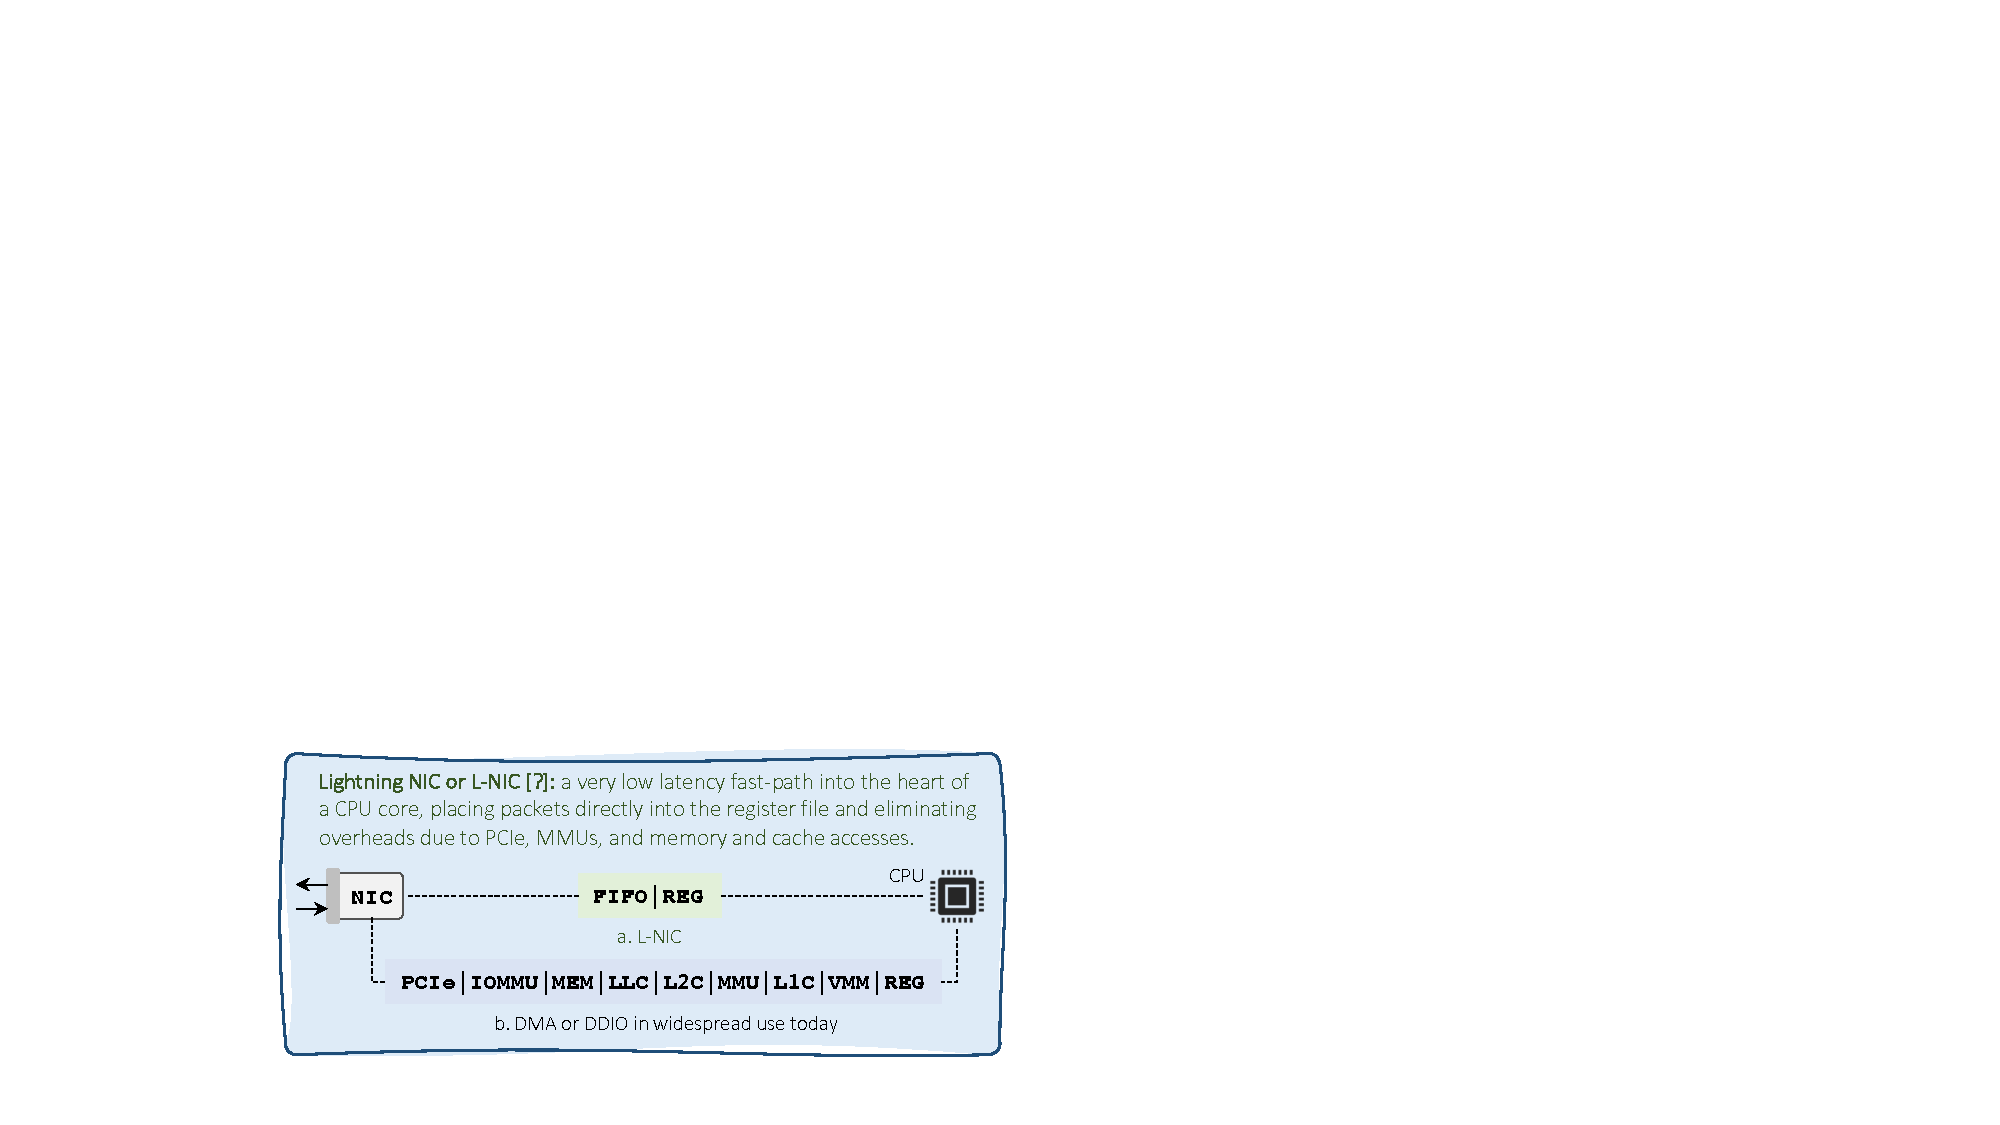
\includegraphics[width=\linewidth]{./figures/lnic-fbox}
  \label{fig:lnic-fbox}
\end{figure}
\shahbaz{add missing citations once the paper is ready.}

More generally, consider a distributed application consisting of $N$ potentially parallelizable tasks, each of which can be executed locally (in $x$ $\mu$s) or on a remote core via RPC (in $r \cdot x$ $\mu$s, where $r \ge 1$). 
If the degree of parallelism, $K$, is the number of issued RPCs (\ie, the number of remote cores), we minimize job-completion time when $(N - K)\cdot x = r \cdot x$ (\ie, $K = N - r$). 
Further increasing the degree of parallelism, $K$, yields no benefit; if we send more RPCs, the local core just sits idle waiting for the RPCs to complete. 
For example, if $r = 10$ (\ie, RPCs take 10 times as long as local execution) then we should send $N-10$ RPCs while executing 10 tasks locally. 
If we reduce latency so that $r=1$, the total job-completion time is reduced by 90\%.  

In practice, RPC completion times, $f_i$, are not fixed, but characterized by a probability distribution, $f_i \in \mathcal{F}$. 
The total job completion time is $(N - K) \cdot x =\max{f_i}$ where $1\le i \le K$. Thus, if we want to improve performance, we must reduce the RPC tail latency $\max{f_i}$. 
This observation is not new and has been the motivation for much recent work~\cite{shinjuku, shenango, rpcvalet}. 

\begin{figure}
  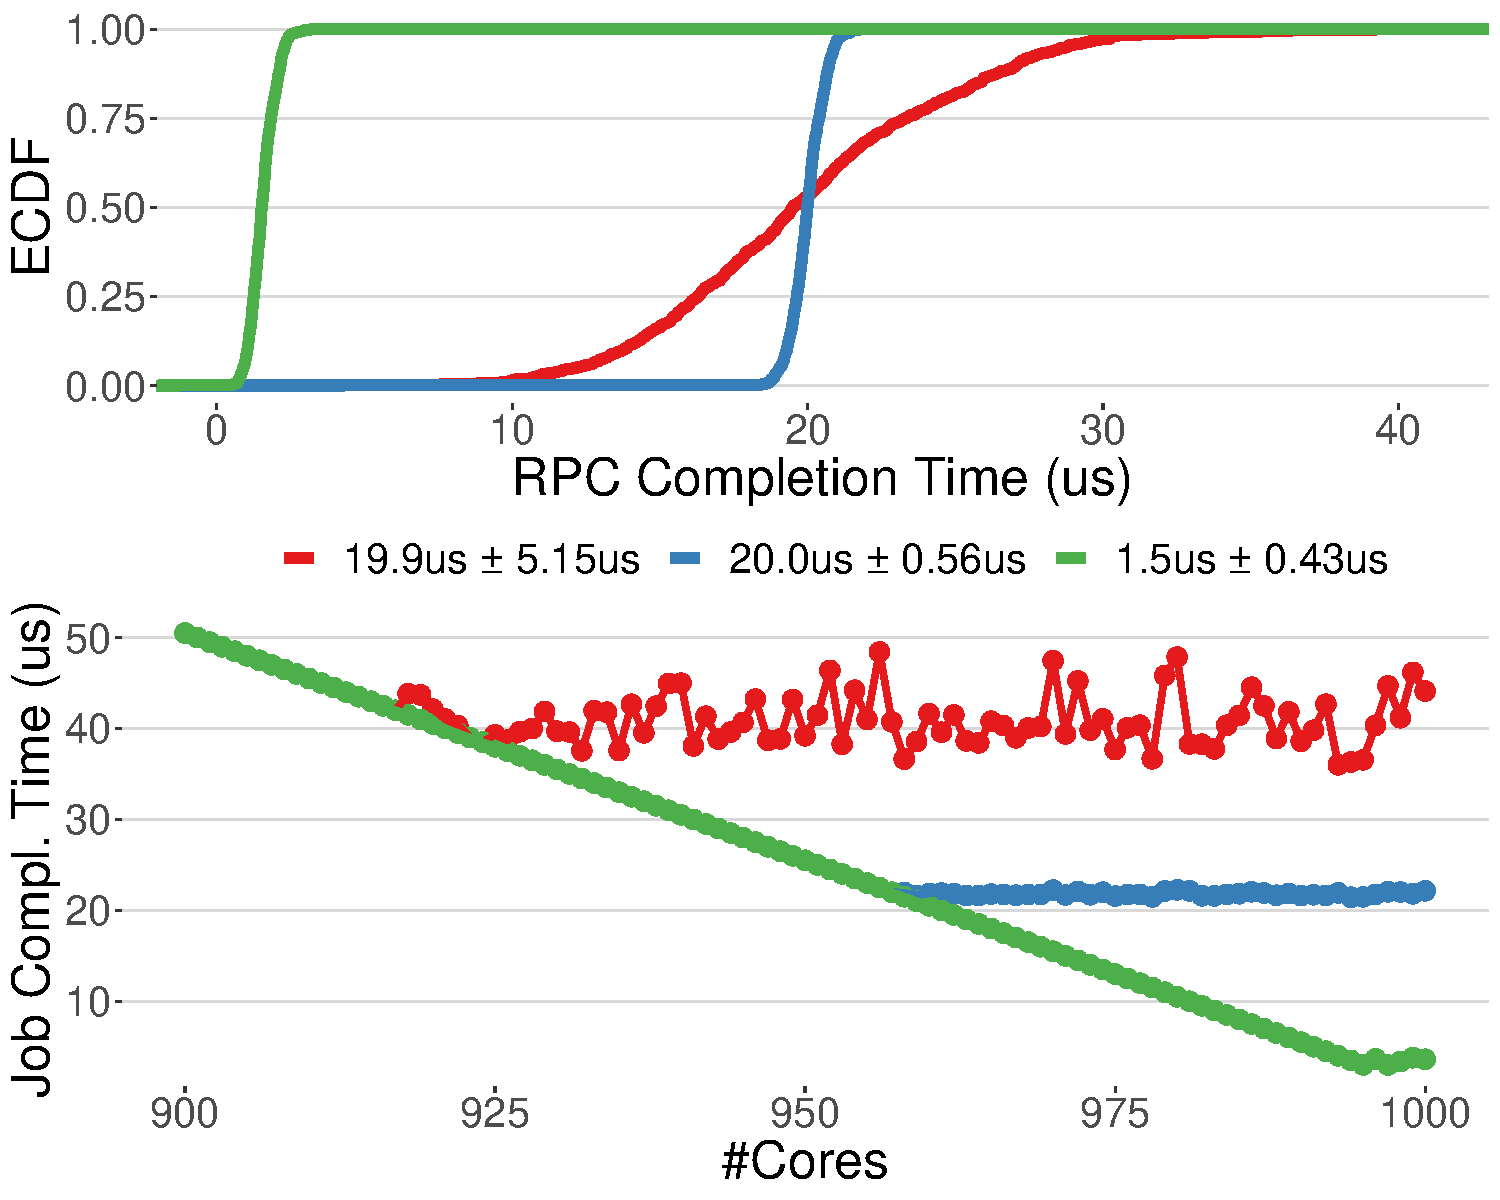
\includegraphics[width=0.9\linewidth]{./figures/nano-comptime}
  \caption{Total job completion time of an example application with 1000 independent tasks (each with \SI{500}{\mu s} processing time) for varying number of cores (\ie, one per RPC) under different RPC completion time distributions.}
  \label{fig:nanoservice-sim}
\end{figure}

The goal of our research is to design, build, and evaluate a domain-specific processor, which we call a {\em \name{}}, optimized for minimizing the completion time of highly-parallel, compute-intensive jobs. The \name{} (\S\ref{sec:nanoPU}) is designed for massive scale-out computing. 
Specifically, millions of \name{}s could be deployed to run what we call {\em nanoservices}: highly distributed, compute-intensive applications that process RPC requests in under \SI{1}{\mu s} using fine-grained, cache-resident threads.

If we are to minimize the average and tail latency of an RPC, we must minimize the latency at every step of the way. 
Starting from when a CPU thread issues an RPC, we must minimize latency through the network stack, through the cache, DRAM and DMA subsystem, through the NIC and onto the wire; across Ethernet links and through switches; and then from the destination NIC through the DMA, DRAM, and cache subsystem; through the network stack, and then wait for the RPC request's target thread to be scheduled for execution by the operating system and for the application to read and process the request.
Most prior work has focused on one aspect of an RPC's latency--for example, low-latency transport layers~\cite{homa, ndp, pfabric} to reduce network congestion and minimize latency through switches, or thread scheduling to make sure an incoming RPC request starts executing promptly~\cite{shinjuku, shenango}. 
Our goal is to reduce RPC response times by at least an order of magnitude from tens or hundreds of microseconds down to approximately \SI{1}{\mu s}. 
This is mostly a networking problem, one that leads us to tackle three questions:

\begin{enumerate}[topsep=0.4\baselineskip, leftmargin=20pt]
    \item {\bf Minimizing {\em average} RPC completion time:} How can we minimize the time that a network message spends between the wire and an application thread?
    This requires minimizing the time through hardware and software. Our approach is to build upon the extremely low-latency {\em Lightning NIC} (L-NIC), described in~\cite{lnic}, in which messages bypass the traditional networking stack, as well as the DMA, DRAM and cache hierarchy entirely, and are placed directly into the CPU register file.
    An arriving RPC can start execution in under \SI{100}{ns}. 
    \item {\bf Minimizing {\em tail} RPC completion time:} How can we limit resource contention for the CPU, memory and network, and minimize the cost of context switching between threads?
    These are the primary causes of variance and hence tail RPC completion times.
    Our approach is to design a thread scheduler into the NIC hardware, as well as to enable the NIC to implement a very low latency hardware transport layer, such as Homa~\cite{homa} or NDP~\cite{ndp}.
    \item {\bf Making it practical:} How can such an extreme approach to hardware and software be practically deployed, with minimal disruption? 
    We have designed and implemented a hardware prototype, based on a RISC-V CPU~\cite{rocket-chip}, that includes a \SI{100}{Gb/s} Ethernet L-NIC CPU interface and a hardware thread scheduler, and we report performance results for real nanoservice applications.
\end{enumerate}

\Cref{fig:nanoservice-sim}, while based on synthetic numbers, illustrates what we aim to achieve.
The first graph shows various distributions of RPC completion times. 
The red graph is intended to be representative of the current state-of-the-art RPC completion times~\cite{eRPC}. The blue graph demonstrates the impact on total application runtime when the standard deviation of the RPC completion time distribution is reduced by an order of magnitude.
If we can drive down the average {\em and} the standard deviation, represented by the green line, then the job-completion time falls linearly as we add cores, until eventually the per-RPC overhead limits parallelism.

% Shahbaz: seems mostly repetitive to what we have already said above, possibly axe it?
%\iffalse
%\nick{The following was in the nanoservices section, but if it stays, it belongs here...} The performance of today's compute-intensive distributed applications is severely limited by the scalability of modern systems, which nanoservices and our proposed NanoPU architecture attempt to address.
%
%For example, consider performing an N-body cosmological simulation of 1 million particles, which is considered to be a small benchmark in the field of astronomy~\cite{changa}.
%This application is designed to simulate the motion of celestial bodies under the influence of gravity.
%It is theoretically possible to parallelize processing for each individual body in the simulation, for instance to compute the force that each body exerts on every other body.
%However, today's parallel programming frameworks (e.g. Charm++~\cite{charm++}) running on modern super computers (e.g. BlueGene/L~\cite{blue-gene-l}) are only able to scale to O(10K) processors~\cite{changa}.
%This means that modern systems are unable to exploit all possible parallelism in the this application, thus wasting opportunities for performance enhancement.
%
%Similarly, consider performing a simple multiplication of two 100x100 matrices, or ray tracing scene with a million objects.
%Each of these operations consist of millions of potentially parallelizable tasks that easily exceed the number of independent compute resources on a modern TPU or GPU.
%
%We believe that these scalability limitations exist for the following reasons:
%\begin{enumerate}
%    \item Large and unpredictable RPC completion times force application developers to prepare for the worst and provision resources accordingly. There is also the well known straggler effect that plagues many modern distributed applications~\cite{tail-at-scale}. Additionally, large overheads for small messages force application developers to batch what would be many small messages into fewer large messages, thus sacrificing opportunities for parallel computation~\cite{anton}.
%    \item Modern network transport protocols are unable to handle massive degrees of incast (e.g. 10K-to-1) without ever overflowing or underflowing the receiver buffer.
%\end{enumerate}
%Our proposed NanoPU architecture is designed to deal with limitation (1), while leaving limitation (2) as a topic for future research.
%\nick{...until here.}
%\fi

In summary, we make the following contributions:
\begin{itemize}[topsep=0.4\baselineskip, leftmargin=20pt]
    \item A new compute framework, called nanoservices (\S\ref{sec:nanoservices}), for highly parallelizable, compute-intensive distributed applications.
    \item The design and implementation of a \name{} (\S\ref{sec:nanoPU}) with a \SI{100}{Gb/s} NIC datapath (\S\ref{ssec:nic-datapath}), a message-based interface directly between the NIC and CPU register file (\S\ref{ssec:niccore-interface}) and a NIC-driven thread scheduler (\S\ref{ssec:thread-scheduler}).
    \item An overview of the hardware mechanisms designed to support a low-latency transport protocol on the NIC (\S\ref{ssec:nic-transport}).
    \item An open-source \name{} prototype (\S\ref{sec:prototype}), based on a RISC-V Rocket Core~\cite{rocket-chip}.
    \item An evaluation of our \name{} prototype against a traditional RISC-V CPU with a DMA-based NIC, for a suite of nanoservice applications (\S\ref{sec:evaluation}). Our evaluation demonstrates that \name{} reduces both average and standard deviation in application-processing times by about $2-10\times$ and $20\times$ respectively.
    \shahbaz{should we be talking in terms of latency or completion times here?}
    \steve{completion times because that's what we are measuring in the evaluations}
\end{itemize}

%\begin{figure}
%  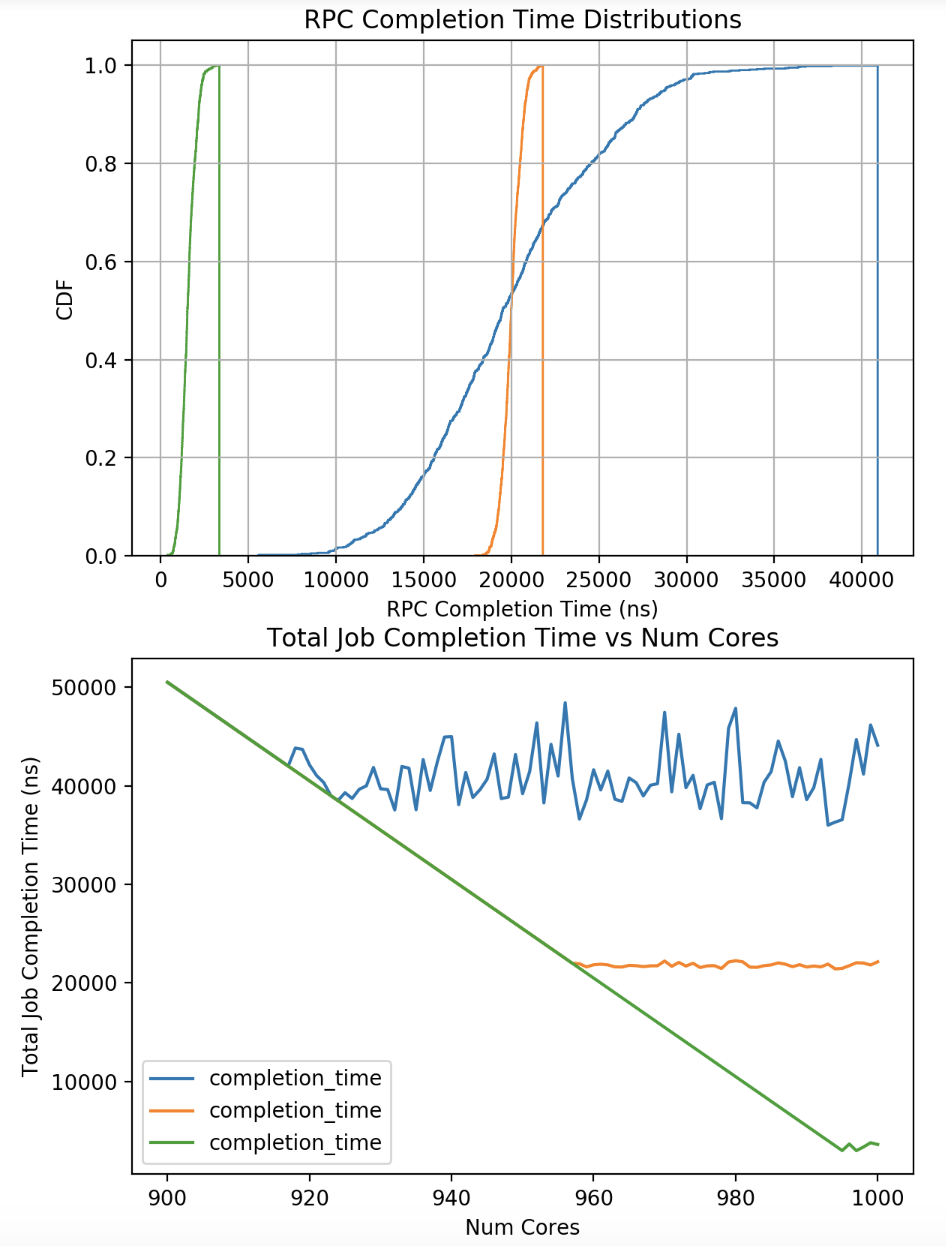
\includegraphics[width=\linewidth]{./figures/nanoservice-sim}
%  \caption{RPC completion time distributions and their corresponding impact on total application runtime for a simple example application.}
%  \label{fig:nanoservice-sim}
%\end{figure}
\section{Nanoservices}
\label{sec:nanoservices}
Nanoservices are a new framework for building compute-intensive, distributed applications with the following three characteristics:

\vspace{0.5pt}
\begin{itemize}[topsep=0.4\baselineskip, leftmargin=20pt]
    \item[\bf C1:] Each application is divisible into compute-intensive {\em nanotasks}, managed by a light-weight {\em nanokernel}.
    \item[\bf C2:] Each nanotask is able to process and respond to network messages in under \SI{1}{\mu s}.
    \item[\bf C3:] The working set of each nanotask fits in the L1 cache.\footnote{L1 cache is typically \SI{256}{kB}--\SI{1}{MB} at the time of writing, including the data and instruction cache.}
\end{itemize}
\vspace{0.5pt}

Figure~\ref{fig:app-frameworks} highlights the key differences between nanoservices and two other major application development frameworks: monoliths and microservices.
We believe that many applications can benefit from the nanoservices framework, including applications such as physical simulations~\cite{barnes-hut, molecular-dynamics}, neural-network inference and training~\cite{tensorflow}, graphics processing~\cite{ray-tracing}, and state-space search algorithms~\cite{state-space-search}.
As we will show in Section~\ref{sec:evaluation}, we can reduce the total application runtime by up to three orders of magnitude if they are implemented using nanoservices.

The central idea is as follows. A nanotask must execute in the shortest, and most deterministic time possible. 
This implies that {\em everything} the nanotask needs must sit in registers and the L1 cache: instructions in the L1 instruction cache, and data (in-progress messages, variables and program state) in registers or the L1 data cache. 
Cache misses are expensive, and the goal is to avoid them---L2 cache and external memory are, ten and one hundred times slower than the L1 cache~\cite{jeff-dean-numbers}, respectively.

Building nanoservices requires more than simply dividing applications into nanotasks that access small amounts of data.
We also need to consider how to quickly and predictably transfer message data between the wire and an application thread, and how to efficiently schedule nanotasks on the available processor cores.
It is not practical to run nanoservices on today's systems, which were designed to support applications that process RPCs in milliseconds, or at best tens of microseconds~\cite{eRPC, perfkit-grpc}, not hundreds of nanoseconds.
Addressing these problems therefore requires hardware changes, which we address with our proposed design, the \name{}, in the following section.

\begin{figure}
  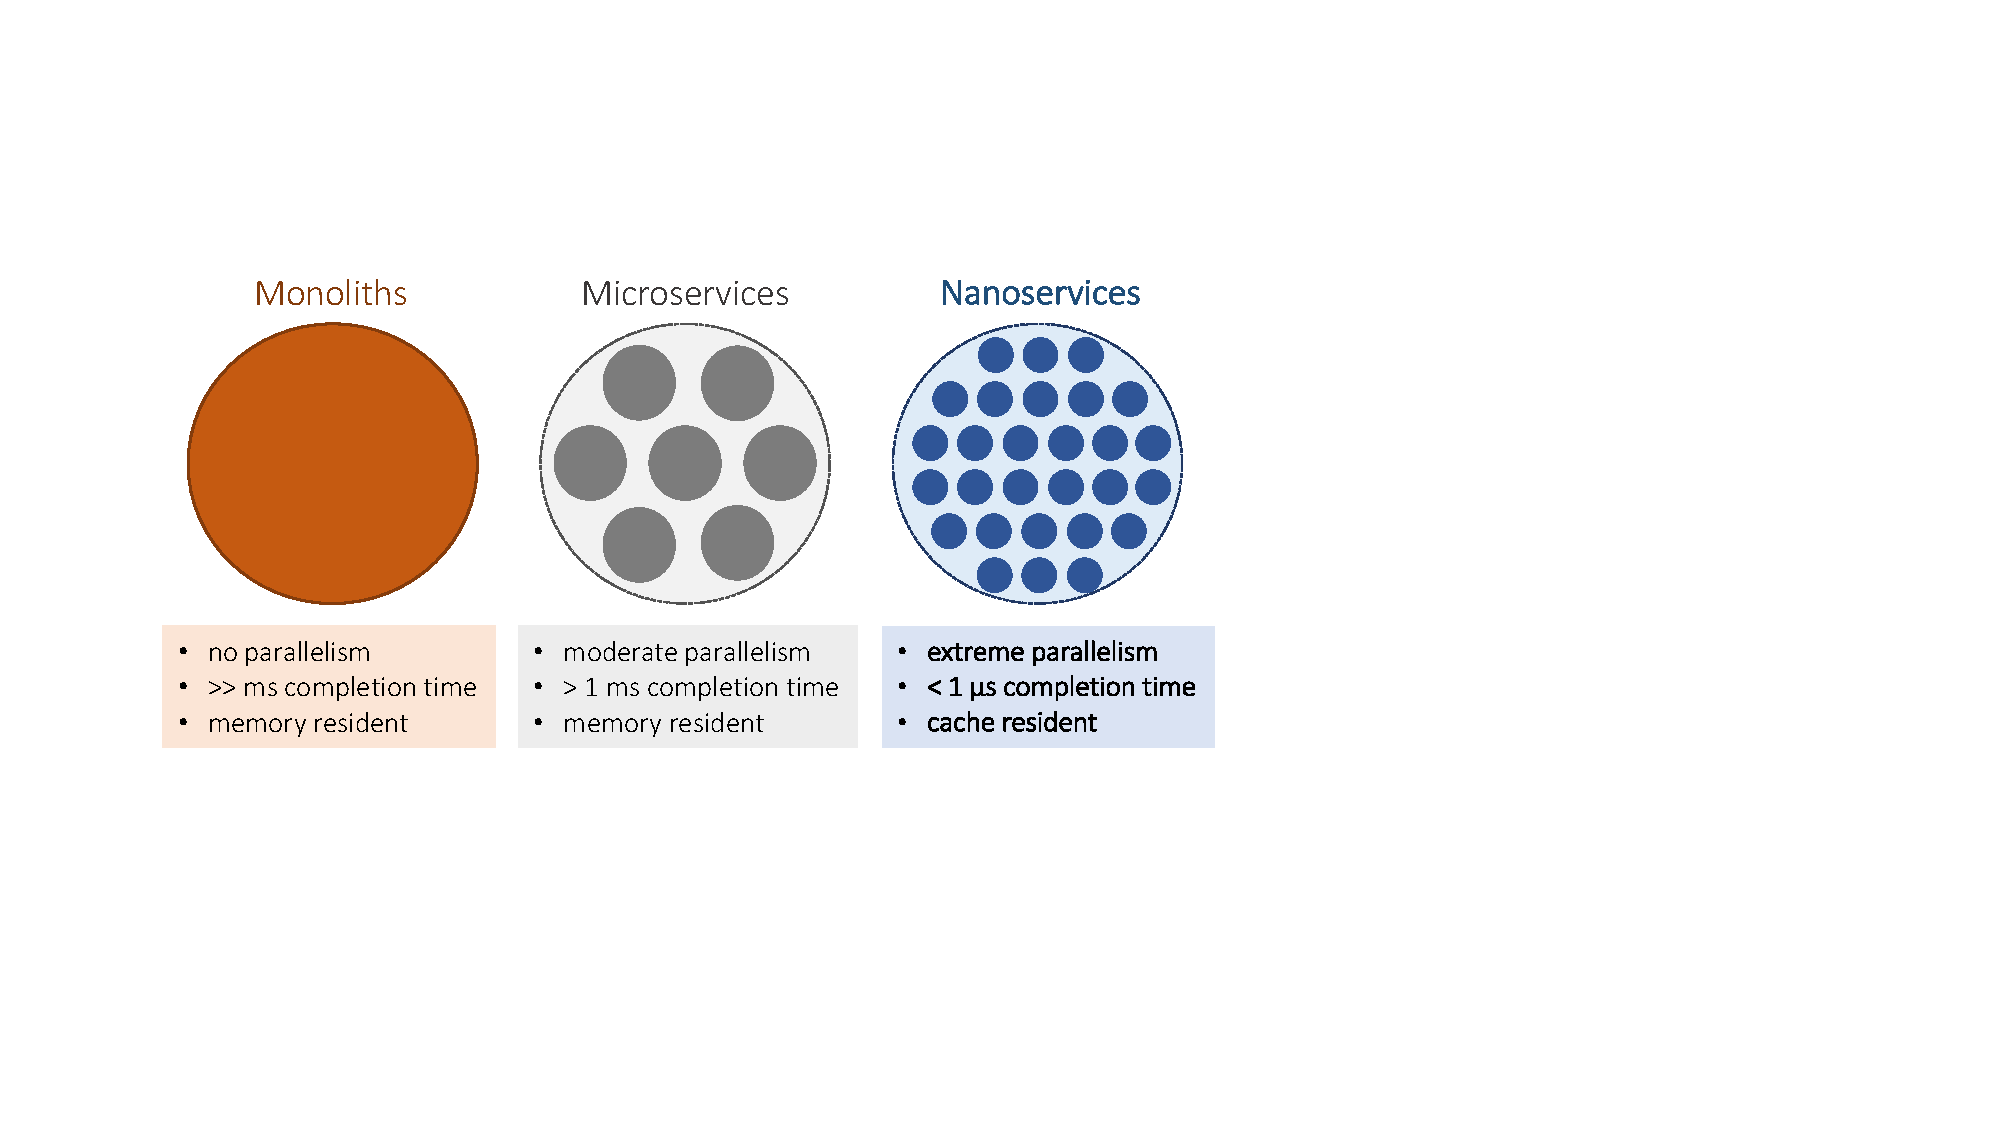
\includegraphics[width=0.9\linewidth]{./figures/app-frameworks}
  \caption{A comparison of key characteristics of {\em nanoservices} vs. monoliths and microservices.}
  \label{fig:app-frameworks}
\end{figure}

\section{The \name{}}
\label{sec:nanoPU}
The \name{} is a new domain-specific processor optimized for running nanotasks---with low average and tail latency---for compute-intensive distributed applications based on nanoservices. 
A \name{} consists of one or more CPU cores and one or more low-latency NICs. 
The CPU cores are slightly modified cores; our design is based on the popular, open-source RISC-V ISA~\cite{riscv}. 
The low-latency NIC is inspired by the recently proposed {\em Lightning NIC (L-NIC)}~\cite{lnic}, a novel approach that terminates the transport layer in hardware, then delivers message data right into the registers at the heart of the CPU core.  
The L-NIC approach minimizes latency (and unpredictability) by bypassing DMA, cache, and DRAM entirely. 
Our \name{} design also adds a novel hardware thread scheduler, to minimize the time (and variability) from when a message arrives until the thread starts processing it.

Figure~\ref{fig:nanoPU} shows a high-level block diagram of a \name{}. 
This particular example shows one network interface shared by three cores, but in general the \name{} is designed to work with any ratio of NICs to cores. 
Depending on the need, it may make sense to build \name{}s with one core per NIC (\eg, for small embedded systems), all the way to hundreds of cores per NIC. 
For example, it would be practical today to design a chip with 500 cores~\cite{celerity, kilocore} and over a hundred \SI{100}{Gb/s} Ethernet interfaces;\footnote{Commercial switch chips exist with $128\times 100$ Gb/s Ethernet MACs today.} in this example, the ratio would be five cores per NIC. 
Of course, many other ratios are possible and the ideal ratio depends on the application, technology, and economics. 

\begin{figure}
  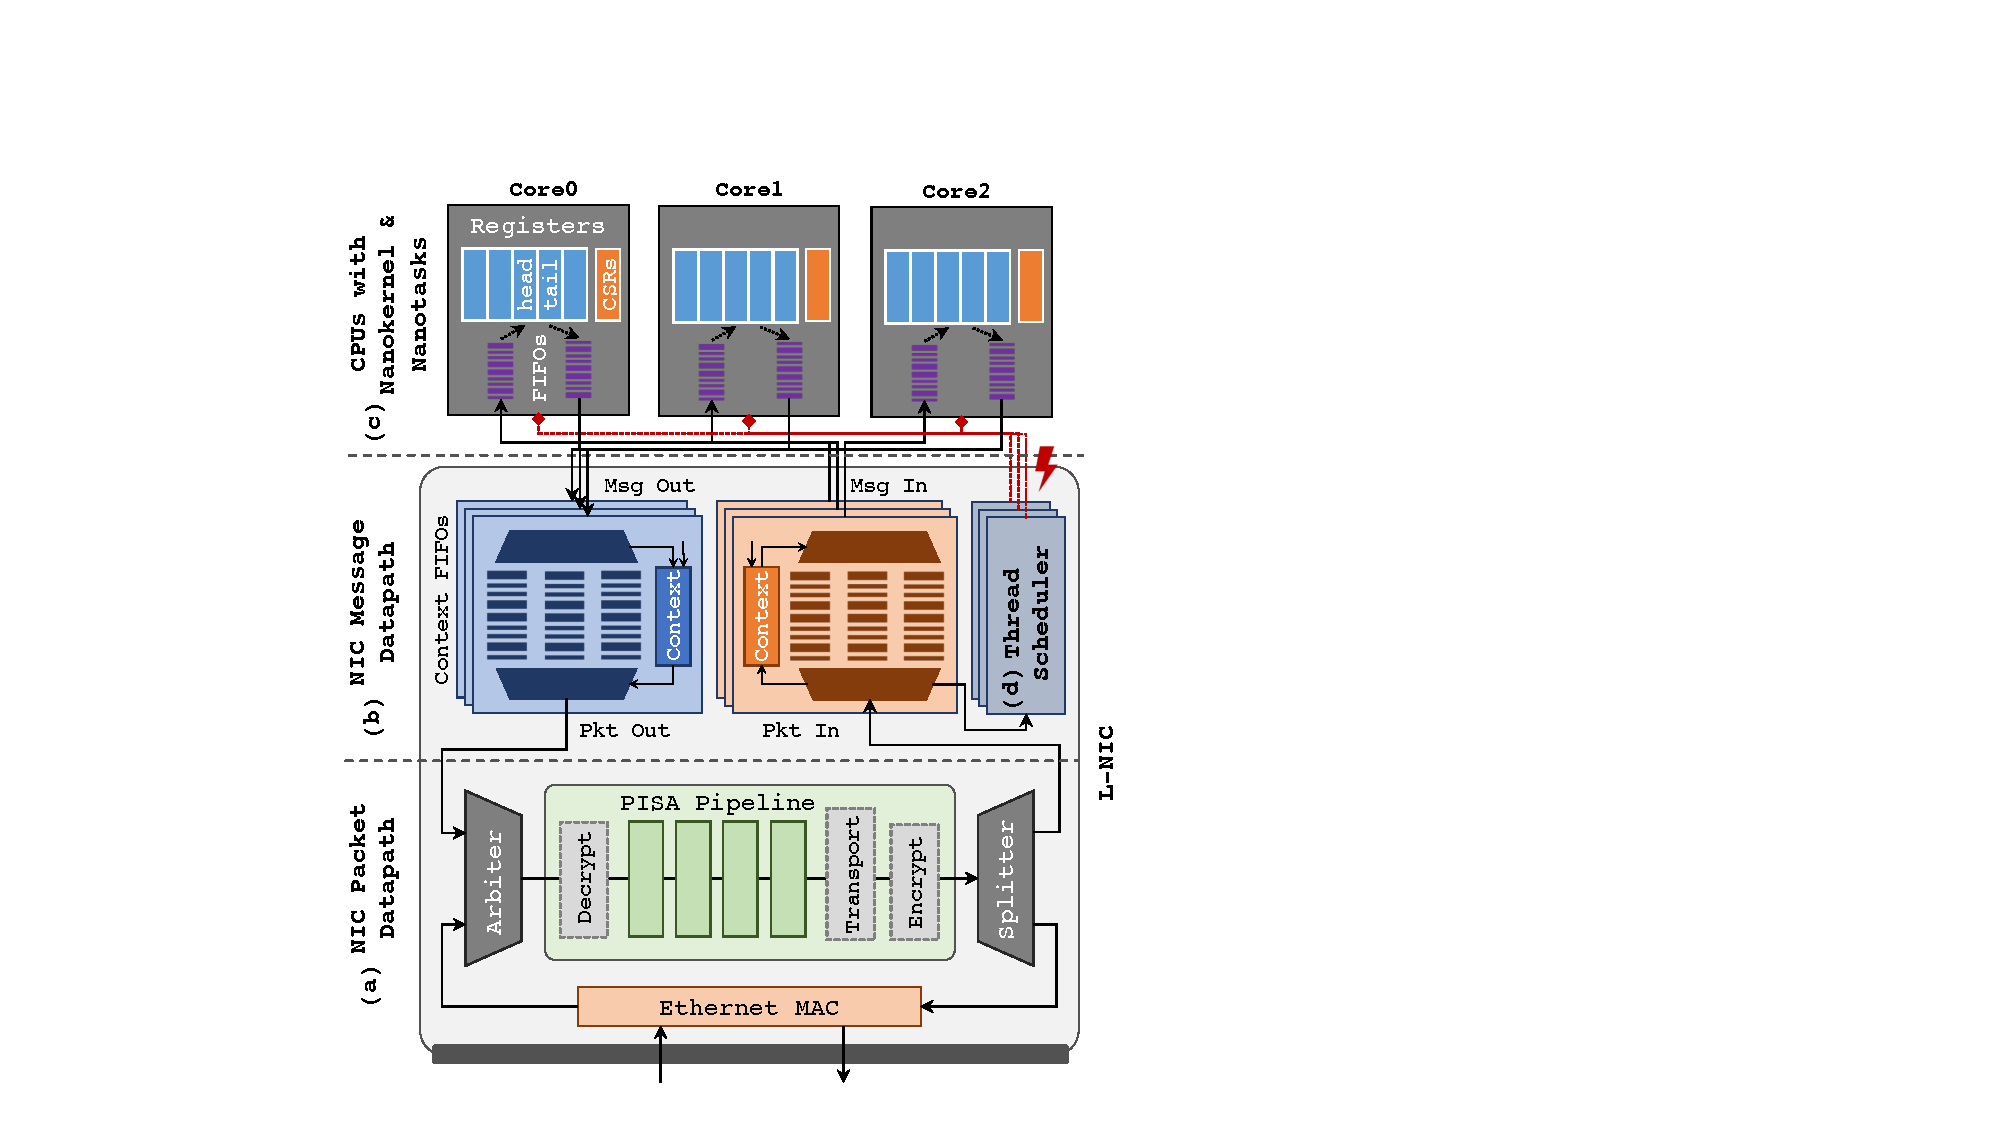
\includegraphics[width=0.95\linewidth]{./figures/nanopu-arch}
  \caption{The \name{} architecture. The NIC includes an event-driven PISA pipeline, and provides an RPC message abstraction to a thread via dedicated RX/TX registers in the CPU. CPU cores run a nanokernel and user nanotasks.}
  \label{fig:nanoPU}
\end{figure}

The \name{} is a domain-specific processor. 
With Moore's Law slowing down, new domain-specific processors are being widely used as accelerators for specific, high-volume workloads, such as graphics~\cite{nvidia-geforce}, machine learning~\cite{tensorflow} and networking~\cite{RMT}. 
While the \name{} is not nearly as radical a departure from a general-purpose CPU as, say, a GPU, TPU or programmable switch (after all, our design relies heavily on an existing core), the \name{} shares the approach of tailoring the chip design for a specific class of applications.\footnote{As an aside, it is only possible to consider prototyping a \name{} in a university because of two recent trends: RISC-V provides a remarkably stable starting point, and the narrow performance gap between the leading edge process (currently \SI{7}{nm}) and the closest already-paid-for process (\SI{16}{nm}) makes it economically feasible to build an interesting \name{}.}

If \name{} is so fast, why are not all CPUs designed this way? 
It is because general-purpose CPUs are optimized for general-purpose workloads, most of which are memory-intensive. 
They are ``load-store'' machines, with memory as a first-class citizen. 
Arriving and departing packet data must pass through the memory subsystem first, on its way in and out of the CPU. 
General-purpose CPUs put memory in the network and attach compute to memory, which makes perfect sense for memory-intensive applications.
Our approach is, instead, to make network messages first-class citizens in their own right, independent of memory. 
Network messages arrive directly into the CPU, without needing to make their way through the memory hierarchy. 
The \name{} is designed to tightly couple compute directly to the network, and then attach memory on the side as needed.

The \name{} has the following key characteristics that we visit, in turn, in the next few subsections: 
\begin{itemize}[topsep=0.4\baselineskip, leftmargin=20pt]
    \item {\bf NIC Packet Datapath:} A programmable event-driven PISA "match action unit" (MAU) pipeline~\cite{event-driven-pisa} on the NIC to process packet headers as they arrive and depart, terminate tunnels, encrypt/decrypt and compress/decompress data; and a low-latency transport protocol in hardware, such as Homa~\cite{homa} or NDP~\cite{ndp}.
    
    \item {\bf NIC Message Datapath:} A very low latency path---just a few clock cycles---from the network right to the very heart of the CPU core---its register file. 
    This reduces latency by 1--2 orders of magnitude; we do not believe there is a lower latency path to a running thread.
    
    \item {\bf Hardware Thread Scheduling:} In addition to moving network messages into the CPU quickly, the \name{} must also make sure that the appropriate application thread is running on the core so that it can start processing messages promptly. For this, \name{} includes a very low-latency, thread scheduler on the NIC and a light-weight nanokernel on the CPU.
\end{itemize}

These characteristics together enable the \name{} to process RPCs quickly and predictably, making it ideal for building compute-intensive, distributed applications.

\subsection{The NIC Datapath}
\label{ssec:nic-datapath}
The NIC datapath processes packets as they enter and leave the network.
Figure~\ref{fig:nanoPU} shows a high-level block diagram of the NIC packet-processing datapath.

The centerpiece of the NIC datapath is an event-driven PISA pipeline~\cite{event-driven-pisa}. 
The original PISA architecture, proposed in the RMT chip~\cite{RMT} and later used by Tofino~\cite{tofino}, is designed for mostly-stateless match-action processing of packet headers; for example for lookups, encapsulation, tunnels and telemetry.
Basic PISA only supports one type of event: the arrival of new packets. 
{\em Event-driven} PISA enhances the basic model to support other event types, such as packet drops, timers and state-dependent events. 
Section~\ref{ssec:nic-transport} describes how an event-driven PISA pipeline can directly support transport protocols in hardware, thus offloading per-packet processing from the CPU. 

The PISA pipeline also performs protocol processing: depending on the loaded P4~\cite{P4} program, it might add and remove Ethernet, IP, VXLAN, GRE, INT~\cite{INT} and transport headers. 
We also program it to add or remove a small per-context header containing the source IP address, a context ID, and message length~\Cref{fig:app-headers}.

\begin{figure}
 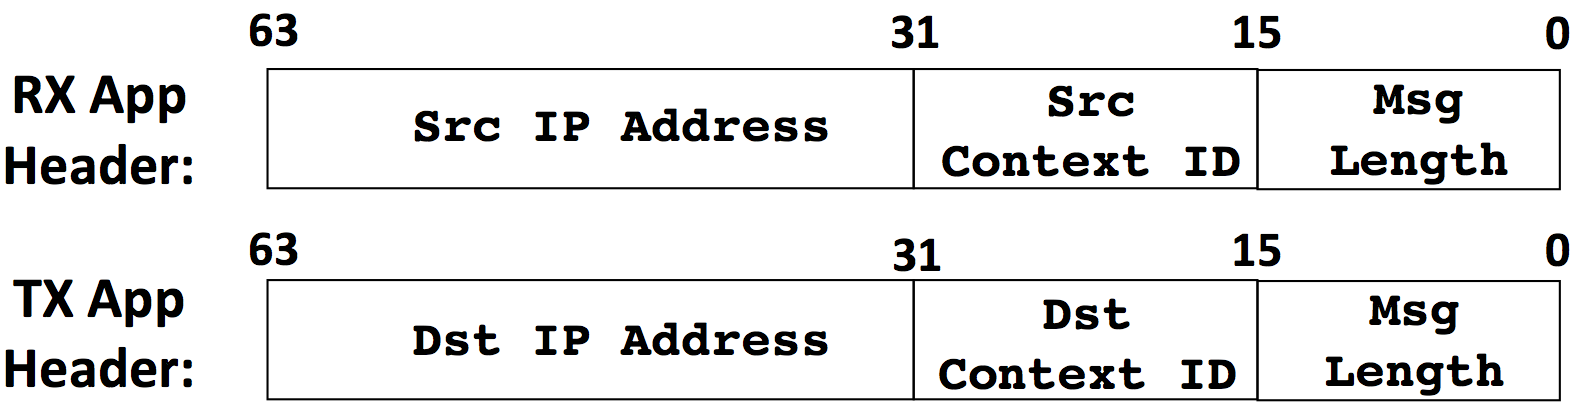
\includegraphics[width=\linewidth]{./figures/app-headers}
 \caption{Application header formats used in the NIC-Core interface.}
 \label{fig:app-headers}
\end{figure}

As others have noted, a P4-programmable PISA pipeline can also be used to accelerate some applications by offloading processing from the CPU (\eg, memory and disk caches~\cite{netcache}, load-balancers~\cite{silkroad}, consensus protocols~\cite{netchain} and firewalls~\cite{p4-firewall}). 
The L-NIC paper~\cite{lnic} describes how a PISA pipeline can accelerate nanoservices to search the Othello state-space.

\subsection{The NIC-Core Interface}
\label{ssec:niccore-interface}
The \name{}'s NIC Message Reassembler and Packetizer, shown in Figure~\ref{fig:nanoPU}, is responsible for assembling arriving packets into a self-contained RPC message, and then queuing the message into its destination nanotask's FIFO, where the message will remain until that nanotask's thread is scheduled. The message then flows, one word at a time, into the core's head register as the nanotask application processes the words. In the egress direction, the Message Reassembler and Packetizer breaks messages into packets before being sending them to the NIC Datapath.

We make two small modifications to allow the CPU core to interface with this layer of the NIC:
\begin{itemize}
    \item Two former general purpose registers (GPRs) are now reserved for a special purpose: one is the HEAD of the network receive queue, and the other is the TAIL of the network transmit queue. Applications must be compiled to avoid using reserved GPRs for temporary storage. Fortunately, \texttt{gcc} makes it easy to restrict register allocation via command line options.
    \item New control status registers (CSRs) are added for out-of-band communication between the CPU and the NIC. These are used to pass nanotask thread IDs and NIC-driven scheduling information between the NIC and the CPU. 
\end{itemize}

The NIC Message Reassembler and Packetizer hardware maintains transmit and receive FIFOs for each nanotask context (i.e. thread) that is currently pinned to the core. The hardware makes sure that the currently running thread only sees (i.e. reads from and writes to) its own per-context FIFO via the HEAD and TAIL GPRs.

The NIC exposes a {\em message} interface to applications running on the core, instead of a more traditional packet interface.
As a result, the \name{} NIC hardware must be responsible for the termination of the transport layer, including breaking messages into packets, ensuring reliable delivery, and processing message reassembly.

To convey relevant transport information, all messages sent or received by an application carry an 8-byte application header whose format is shown in Figure~\ref{fig:app-headers}. Applications must write the message's destination IP address, destination nanotask context ID and message length at the start of all outgoing messages. (Including the message length allows the NIC to determine when the application has finished writing a complete message.) Similarly, all incoming messages read by any application will begin with the message's source IP address, source nanotask context ID, and message length.

% \begin{figure}
%   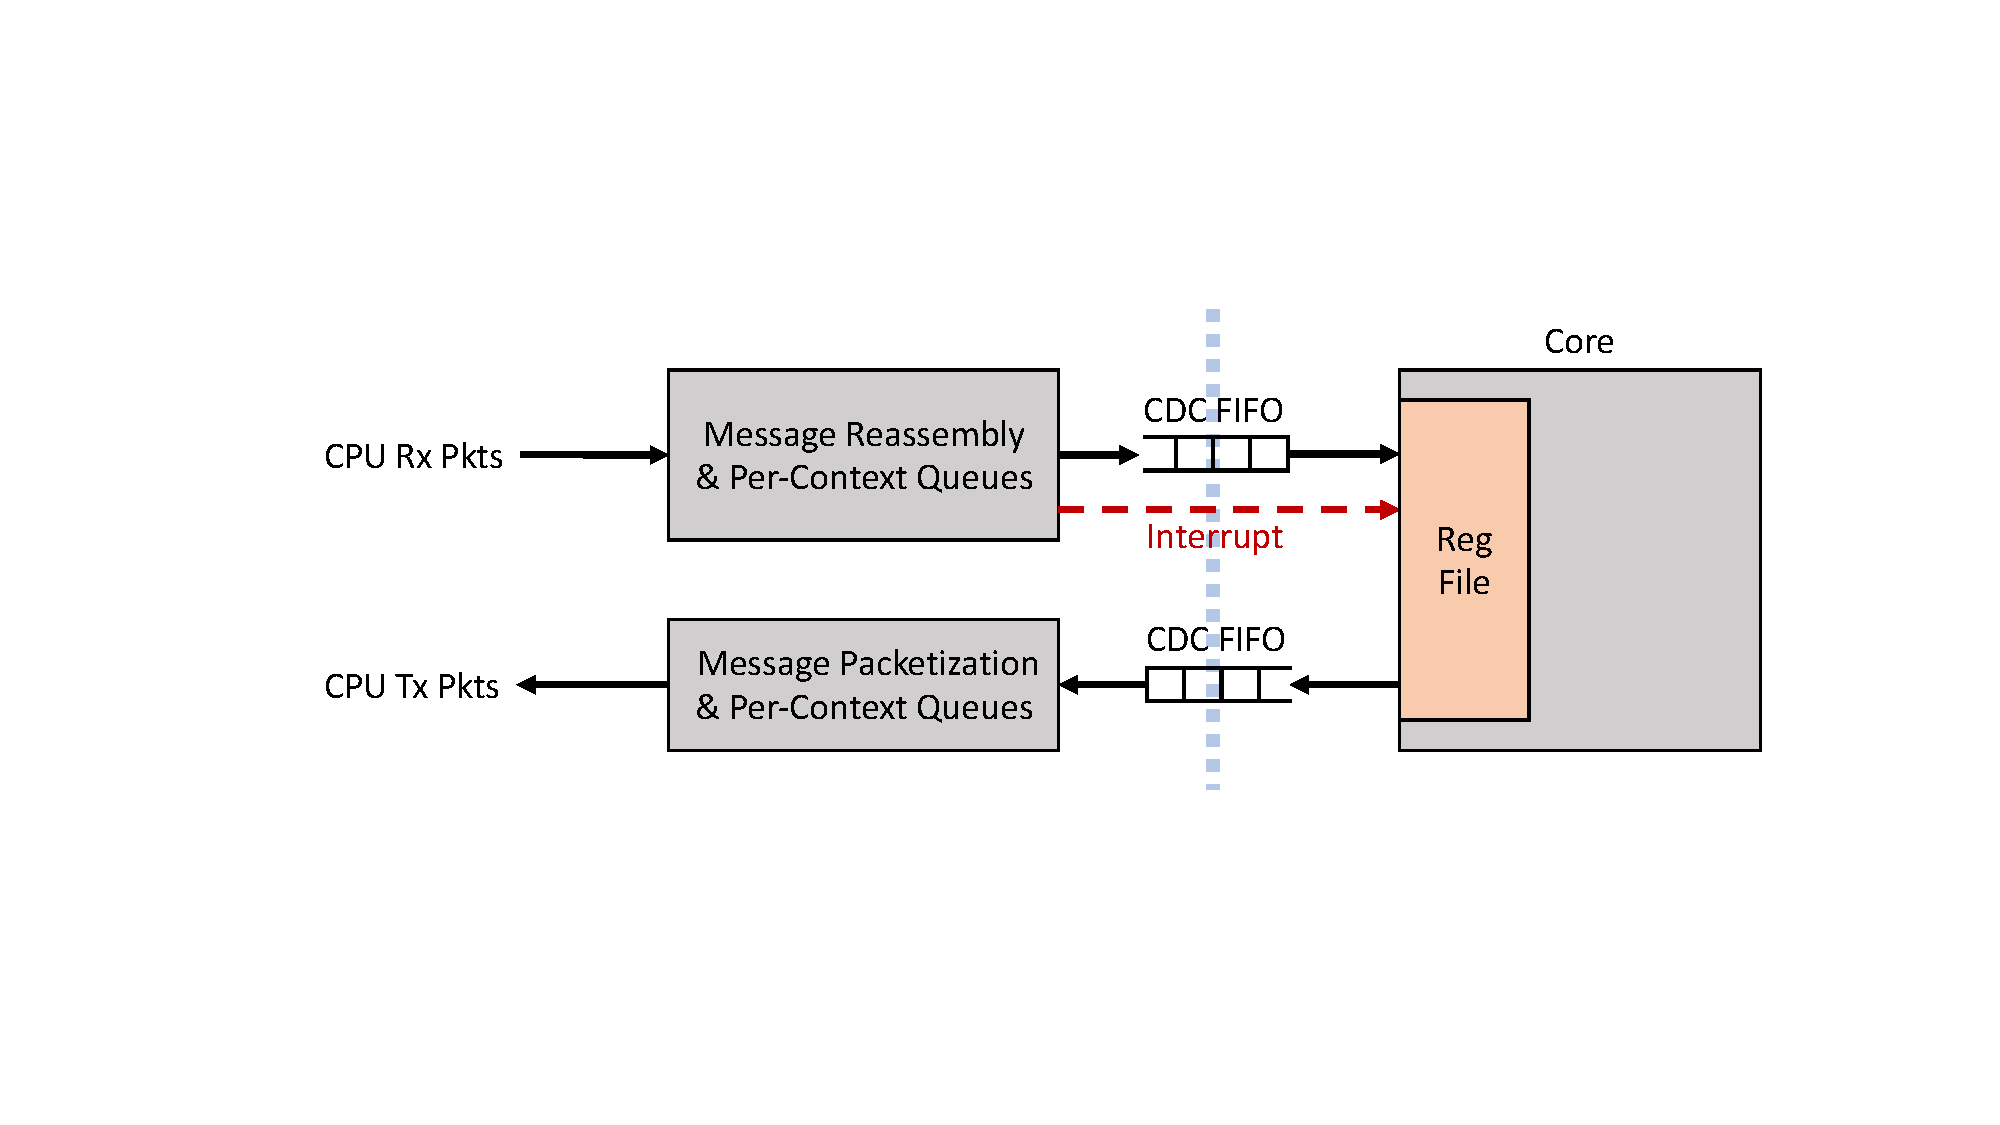
\includegraphics[width=\linewidth]{./figures/NIC-Core-Interface}
%   \caption{Block diagram of the \name{}'s NIC-Core interface.}
%   \label{fig:NIC-Core-Interface}
% \end{figure}

{\lstinputlisting[language=riscv]{code/loopback.S}
\vspace{-20pt}
\captionof{lstlisting}{Loopback with increment: A simple RISC-V \name{} assembly program to register a context \& priority with the NIC, wait for a 16B message to arrive then increment values during loopback from HEAD to TAIL FIFOs..}
\label{lst:asm}}

%\lstinputlisting[caption={Loopback with increment: A simple RISC-V \name{} assembly program to register a context \& priority with the NIC, wait for a 16B message to arrive then increment values during loopback from HEAD to TAIL FIFOs.}, label={lst:asm}]{code/loopback.S}

To illustrate how a \name{} interacts with its NIC, Listing~\ref{lst:asm} shows a simple loopback$+$increment program in RISC-V assembly language.  The program continuously reads 16 byte messages (consisting of two 8 byte integers) from the network, increments the integers, and sends the messages back to their sender. The program is described in more detail below.

The \textbf{\texttt{entry}} procedure registers a nanotask context ID with the NIC using the \texttt{lcurcontext} CSR (in the example, it sets the context ID to be 0). The procedure also sets the priority of the context (again to 0, the most urgent) using the  \texttt{lcurpriority} CSR. It then executes the command by setting the \texttt{lniccmd} CSR to value 1. \texttt{lniccmd} is a bit vector used by supervisor mode software to send commands to the NIC--in this case, it is used to tell the NIC to allocate an RX and a TX queue for context ID$=0$ with priority level$=0$. The \texttt{lniccmd} CSR can also be used to remove context IDs or to update the priority level.\footnote{Although the \texttt{lcurcontext}, \texttt{lcurpriority} and \texttt{lniccmd} CSRs convey hardware commands, they serve a similar purpose to opening or closing a socket in a traditional operating system.}

The \textbf{\texttt{wait\_msg}} procedure waits for a message to arrive in the RX queue by polling the \texttt{lmsgsrdy} CSR until it is set by the NIC, indicating that the context has messages to process. While it is waiting, the application tells the NIC that it is idle by setting the \texttt{lidle} CSR during the polling loop. The NIC thread scheduler uses the idle signal to evict waiting threads and, instead, schedule a new thread with a new message waiting to be processed. 

The \textbf{\texttt{loopback\_plus1\_16B}} procedure simply swaps the source and destination addresses by moving the application header (the first word of every message) from the head register (\texttt{t5}) to the tail register (\texttt{t6}), shown on line 20. It then increments every integer in the received message, appends them to the message being transmitted, and waits for the next message to arrive.

Applications that use variable length messages can use the message length (in the application header) to read the correct number of words from the network RX queue. If an application reads an empty RX queue, the resulting behavior is undefined - similar to reading an uninitialized variable.
\subsection{NIC-Driven Thread Scheduling}
\label{ssec:thread-scheduler}
In some specialized applications, thread scheduling might not be needed: Big HPC applications, for example, might pin every nanotask to a dedicated core for the duration of a run.
But this would not work for a cloud provider who needs more economical sharing of \name{}s by multiple nanoservice applications.
Nanotask threads will therefore need to be switched in and out frequently, and context switches must be extremely fast, else we will lose all the low latency benefits of nanoservices.

If \name{} relied on software scheduling it would be too slow. 
The fastest best-of-breed software schedulers use 5$\mu$s timer interrupts~\cite{shinjuku, shenango} which are much too slow for our $<1\mu$s nanotasks.
And so, instead, the \name{} decides which thread to run next in hardware on the NIC (\Cref{fig:nanoPU}d), then tells the CPU core. 
The NIC keeps track of the highest-priority nanotask with messages to process and interrupts the CPU to initiate a context switch under two conditions:

\begin{enumerate}
    \item A message arrives for a higher priority context than the one currently running on the core.
    \item The current context tells the NIC it is idle, and the NIC has messages for another context to process. 
    This condition prevents an idle high-priority context from starving a low-priority context with messages waiting to be processed.
\end{enumerate}

\Cref{fig:nic-scheduler} shows what happens when a message arrives for a higher-priority context than the one currently running on the core. 
In step \ballnumber{a}, the arriving message is enqueued into the RX queue for the high-priority context.
In step \ballnumber{b}, the thread scheduler tells the CPU that a high-priority message is waiting by updating the \verb|ltargetcontext| CSR and firing an interrupt.
The interrupt causes a trap into the nanokernel, which then reads the \verb|ltargetcontext| CSR and performs a switch to the high-priority context in step \ballnumber{c}, updating the \verb|lcurcontext| CSR.
At this point, the high-priority context is running on the core and is able to process the message in its RX queue.
When the high-priority context finishes processing the message, it tells the NIC that it is now idle by writing to a dedicated CSR called \verb|lidle|.
The NIC then initiates a context switch back to the low-priority context because it still has messages to process.

\shahbaz{will update Figure~\ref{fig:nic-scheduler} to contain the relevant CSRs}

\begin{figure}
  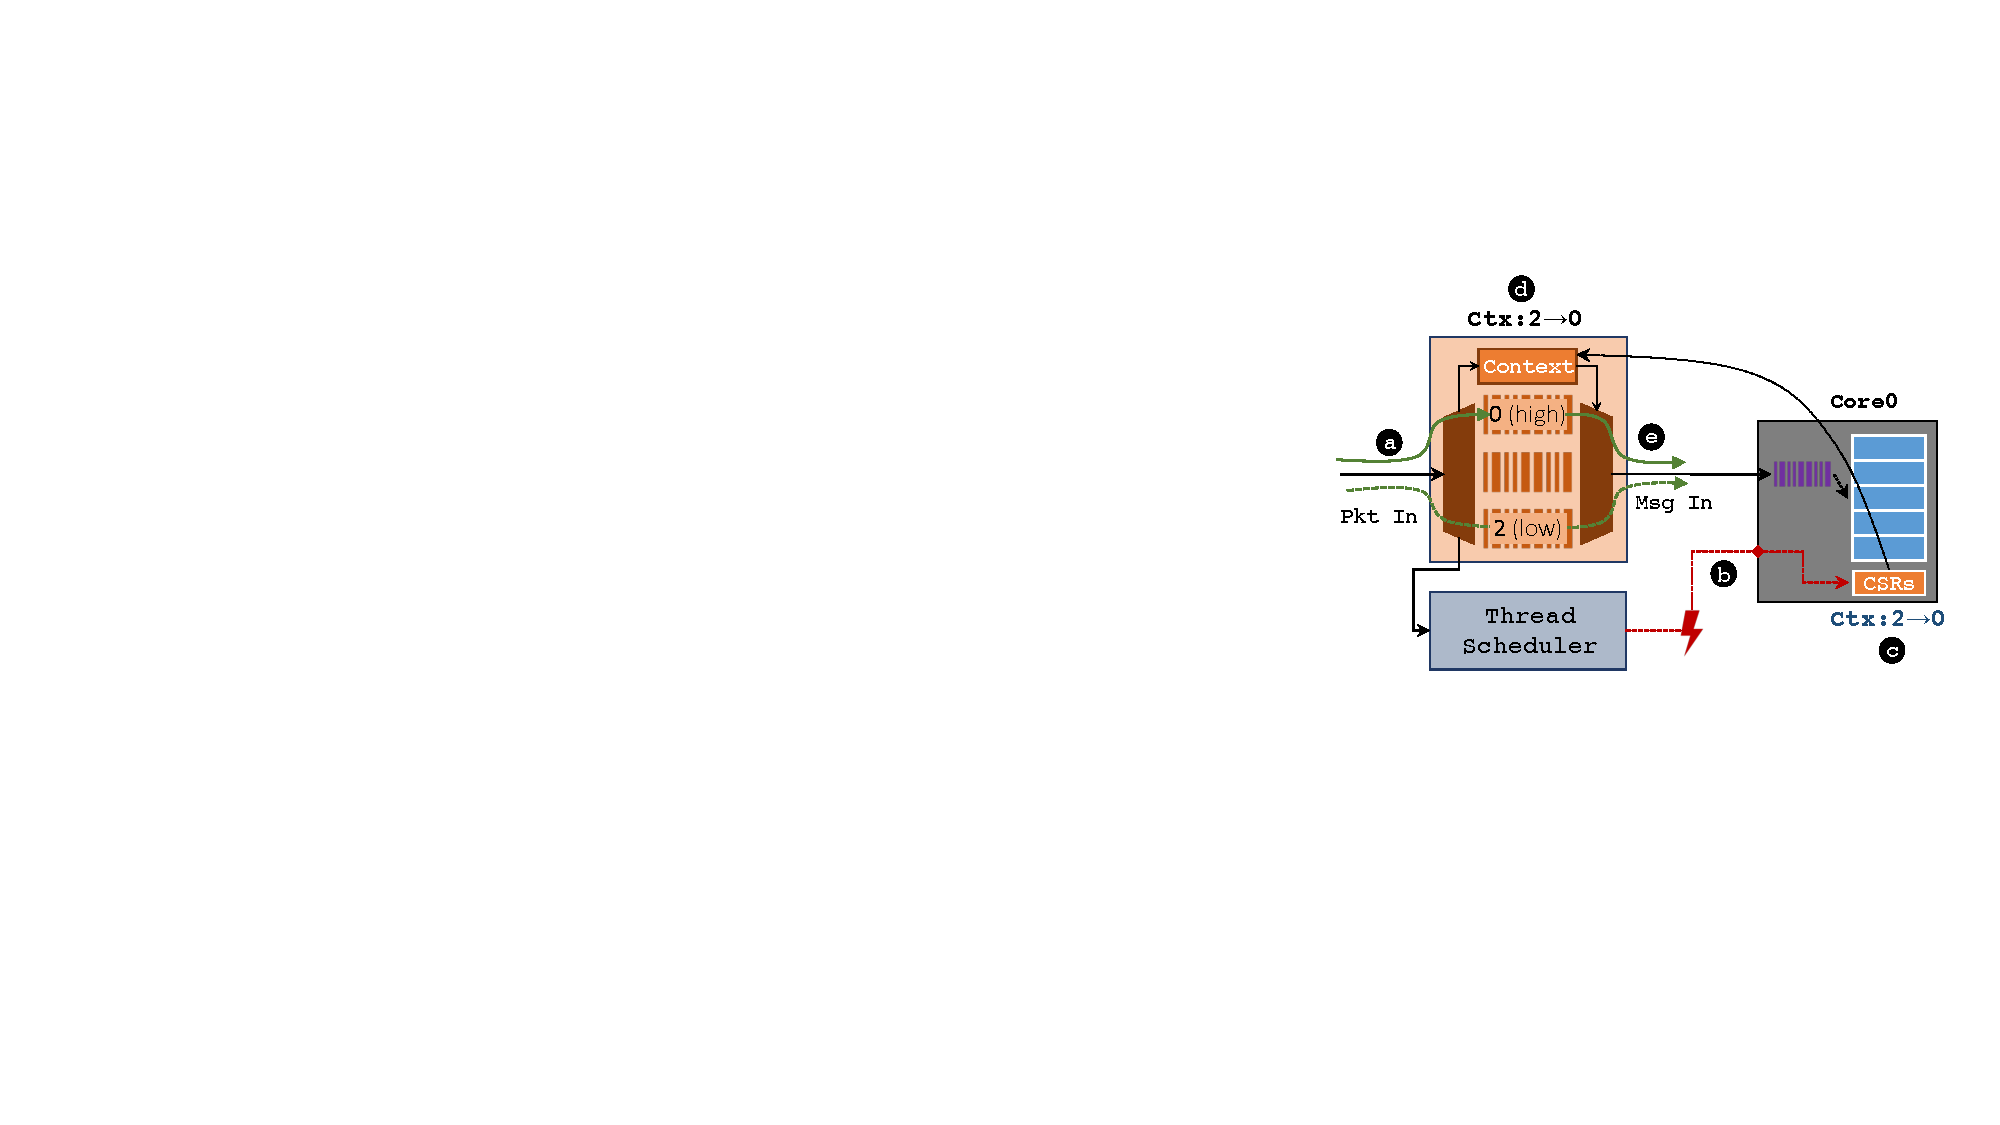
\includegraphics[width=0.8\linewidth]{./figures/thread-sched}
  \caption{The steps that occur when a low-priority thread running on a core is preempted by a higher-priority context.}
  \label{fig:nic-scheduler}
\end{figure}
\subsection{Terminating Transport in the NIC}
\label{ssec:nic-transport}
If the \name{} is to meet our aggressive latency target of $<1\mu$s from when an RPC message arrives over Ethernet until a response is sent back out, there is clearly no time to run a traditional transport networking stack in software. Therefore, \name{} runs a low-latency transport protocol in hardware, in the NIC, with support from the NIC's programmable pipeline. Note that transport protocols for low-latency applications (e.g., DCQCN for RDMA) are already fully implemented in hardware~\cite{cvl,connectx6} on state-of-the-art high-speed NICs available in today's market, vouching for the feasibility of a fully-offloaded transport protocol running in hardware.

We, however, don't mandate a specific transport protocol in this paper because we seem to be entering an era when different cloud providers prefer different transport protocols~\cite{timely,hpcc,dcqcn}. Instead we aim to provide some choices, within our tight latency budget.

The NIC therefore places minimal constraints on the transport protocol, while providing programmable hardware blocks to allow some choice by the network owner. We assume that the transport layer provides a reliable message abstraction to each thread, as well as network congestion control. It therefore must handle retransmissions and decide when packets should be sent. To guide our design, we assume it must be possible for the NIC to be programmed to implemented Homa~\cite{homa} and NDP~\cite{ndp}. Between them, they mandate most of the building blocks we need, including reliable transmission, immediate startup rate, receiver driven scheduling, a message abstraction to the CPU, and data-trimming (in the switches).

We observe that realizing a transport protocol in hardware requires the following functions in the programmable pipeline of a NIC.

\begin{itemize}
    \item Timers and timer-based event processing logic to realize various timer-based state transitions, such as retransmissions and timeouts.
    \item Pacers to rate-limit individual flows.
    \item Flow state machine to maintain per-flow state, including current rate or congestion-window size, sequence and acknowledgment numbers, connection-establishment status, counters, etc.
    \item Packetization/retransmission buffer to break a message into packets and hold packets until they are acknowledged by a receiver.
    \item Reordering buffer to handle out-of-order delivery of packets.
    \item Packet generators to realize receiver-driven transport protocols that keep generating credit packets for senders.
\end{itemize}

The event-driven PISA pipeline~\cite{event-driven-pisa} already provides most of the mechanisms we need for sophisticated stateful operations (\eg, state machines, timer events and packet generation), and can be extended to add support for message reassembly and retransmit buffers~\cite{schuehler2004modular, intel-rapidio}. Because nanoservice messages sizes will be very small, the amount of SRAM needed to realize these buffers will be sufficiently small for a cost- and power-efficient hardware implementation. With these mechanisms, we believe the \name{} can run a complete transport stack on the NIC with very low latency. While we have a design for each of these building blocks, we will explain the details of those in our follow-on paper.

\iffalse
The key components that enable the NIC to terminate a transport protocol are described below.

The \textbf{event-driven PISA pipeline~\cite{event-driven-pisa}} is a programmable data-plane architecture that enables us to write programs that process data-plane events in the background of data packet processing, that is, without affecting the rate at which data packets are processed.
It does this by scheduling and aggregating memory accesses.
This mechanism helps to enable transport logic processing which must perform more sophisticated stateful operations than basic packet forwarding.

The \textbf{timer event generation module} is a hardware mechanism within the aforementioned event-driven PISA pipeline that is able to maintain $N$ timers (e.g. one per active message or one per active RPC).
The timer module supports the following three operations per-timer:
\begin{itemize}
    \item Schedule - add a new timer
    \item Reschedule - restart an existing timer
    \item Cancel - remove the state associated with an existing timer
\end{itemize}
These timer events are processed in the background of data packet processing and are used to determine when a data packet retransmission must be sent or when a message (or RPC) has expired and its state must be cleaned up.

The \textbf{programmable packet generation module} is used to generate acknowledgement and/or message completion packets.

The \textbf{packetization buffer} stores messages sent from the CPU and generates packets that are subsequently processed by the event-driven PISA pipeline before being transmitted.
It also supports retransmitting data packets within a message when a packet drop is detected.

The \textbf{message reassembly buffer} is able to reassemble potentially multi-packet messages with duplicate packets into a single message that is then delivered to the appropriate RX queue for the destination context.
\fi

\section{\name{} Prototype}
\label{sec:prototype}
In order to evaluate the expected performance of a \name{}, we built a prototype in Chisel~\cite{chisel} and C on top of the open source RISC-V Rocket Core system~\cite{rocket-chip} and evaluated performance using cycle-accurate hardware simulations~\cite{verilator}.

Figure~\ref{fig:nanoPU-prototype} shows a high-level block diagram of the prototype's most relevant components.
The prototype implements the main components of the NIC described in \S\ref{sec:nanoPU} and connects it to a slightly modified RISC-V Rocket core.
The prototype implements the following aspects of the \name{}:
\begin{itemize}
    \item The NIC Datapath, without a hardware transport protocol, encryption/decryption or MAC processing.
    \item The NIC-Core Interface, including small changes to the core required to add the fast path into the register file.
    \item The NIC hardware thread scheduler and nanoKernel.
\end{itemize}
Since the NIC and core run at the same clock rate in our prototype, we have no need for clock domain crossing (CDC) FIFOs in the NIC-Core Interface. \steve{Check if we are still describing the CDC FIFOs in the NIC-Core Interface description}
Furthermore, since the prototype does not implement a transport protocol, we assume that all messages sent and received by the applications consist of a single Ethernet packet, which we believe will be true for the vast majority of nanoservice applications.

To provide a useful reference, we compare the performance of our \name{} prototype to a RISC-V Rocket Core with a traditional DMA-based NIC called IceNIC~\cite{firesim}.
Figure~\ref{fig:icenic-prototype} depicts a block diagram of the IceNIC RISC-V system.
IceNIC behaves in a similar fashion to Intel DDIO based NICs.
That is, it uses DMA to move network packets directly between the NIC and the CPU's last level cache.
Since the IceNIC RISC-V design is an integrated solution, it does not include a PCIe bus--thus we expect it to exhibit lower latency than a typical modern NIC.

We made one change to the original RISC-V IceNIC design to make up for the RISC-V ISA's omission of byte reversal instructions.
Since this operation is extremely common in network applications, and because Intel processors have hardware support for this type of operation, we added these instructions to our RISC-V processor in order to accelerate IceNIC applications.
This changes allows us to obtain a more fair performance comparison with our \name{} prototype.
These instructions are not needed for \name{} applications because the NIC swaps the byte order of message data before making it available to the application.

\begin{figure}
  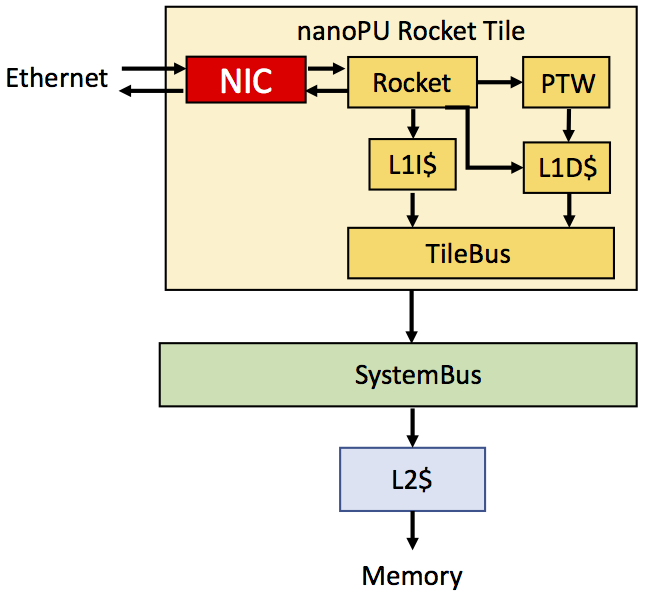
\includegraphics[width=0.75\linewidth]{./figures/nanoPU-prototype}
  \caption{Block diagram of \name{} RISC-V prototype.}
  \label{fig:nanoPU-prototype}
\end{figure}

\begin{figure}
    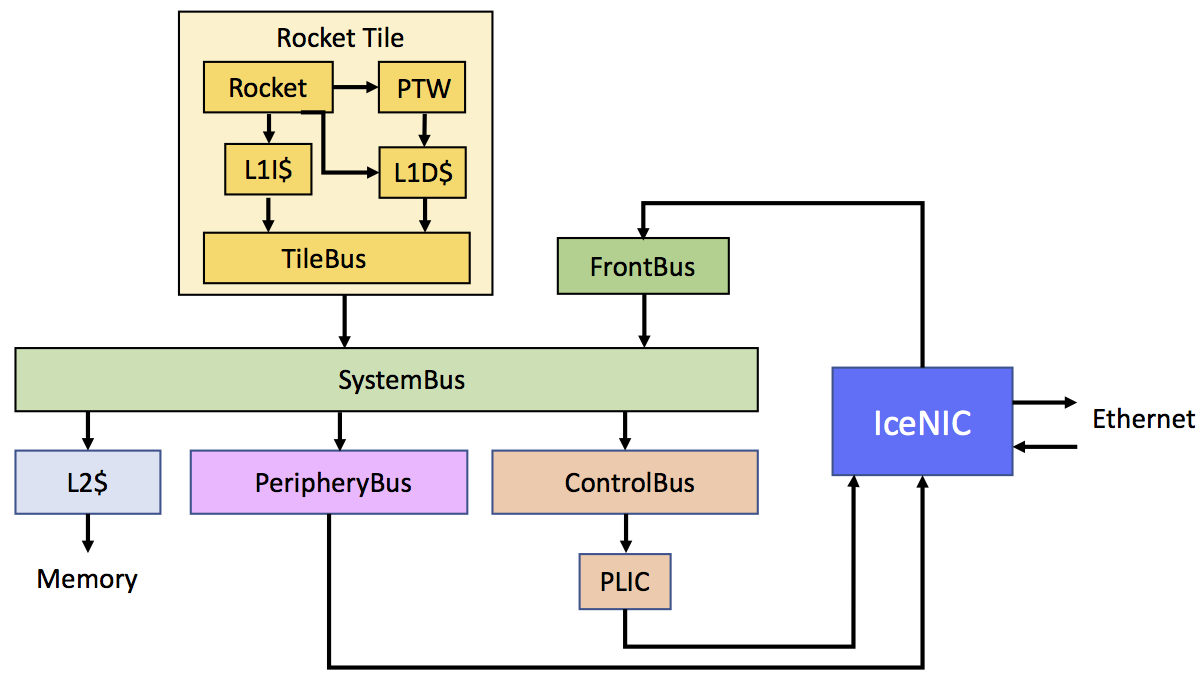
\includegraphics[width=\linewidth]{./figures/icenic-prototype}
    \caption{Block diagram of a traditional RISC-V system with a DMA-based NIC called IceNIC.}
    \label{fig:icenic-prototype}
\end{figure}
\section{Evaluations}
\begin{itemize}
    \item We built a NanoPU prototype on top of the open source RISC-V Rocket Core. Cite chipyard XXX.
    \item For the prototype we focused on building the NanoPU NIC datapath, NIC-Core interface, and a minimal operating system (the NanoKernel).
    \item Our prototype does not implement a full NanoPU:
    \begin{itemize}
        \item It does not make any modifications to the memory hierarchy.
        \item It does not implement any encryption or decryption.
        \item The NIC and the core run at the same clock rate, hence the CDC FIFOs are not included.
        \item The prototype assumes all messages consist of a single packet. It does not implement a reliable transport protocol.
    \end{itemize}
    \item We will assume a 3 GHz clock for our RISC-V prototype in order to report performance numbers, because this is a typical clock speed for a CPU. \steve{Should we report performance numbers in terms of clock cycles or Gbps and nanoseconds?}
    \item Probably need to include a description of how well we believe IceNIC represents a modern state-of-the-art NIC.
\end{itemize}

\subsection{Microbenchmarks}
This section describes a set of microbenchmarks that characterize various aspects of the NanoPU architecture.

\paragraph{Timing Analysis.} We synthesized both our NanoPU RISC-V prototype as well as a standard RISC-V core with a traditional NIC (IceNIC) to a modern FPGA (Xilinx Ultrascale+) in order to analyze the critical paths in each design. We found that the critical path in both designs is in the L2 cache, and hence our NanoPU prototype is able to achieve the same clock rate as a traditional RISC-V system.

\paragraph{Basic Latency/Throughput Performance Analysis.} The latency of the NanoPU's TX path is 11 cycles for a single word message, which is measured from the cycle when an application writes the word to when the word is placed on the network (not including the MAC processing). The corresponding latency of the RX path is 6 cycles. Figure~\ref{fig:loopback-latency} shows the loopback latency for various packet lengths for both our NanoPU prototype and the traditional DMA-based IceNIC.

Table\ref{tab:throughput} shows the TX and RX throughput for 64B packets for both our NanoPU prototype and IceNIC. 

\begin{table}[]
\begin{center}
\begin{tabular}{|c|c|c|c|c|}
\hline
                & \textbf{RX bytes/cycle} & \textbf{RX Gbps} & \textbf{TX bytes/cycle} & \textbf{TX Gbps} \\ \hline
\textbf{NanoPU} & 3.01                    & 72               & 7.65                    & 185              \\ \hline
\textbf{IceNIC} & 0.58                    & 14               & 1.16                    & 28               \\ \hline
\end{tabular}
\caption{TX and RX throughput achievable by both our NanoPU prototype and IceNIC.}
\label{tab:throughput}
\end{center}
\end{table}

\begin{itemize}
    \item TX/RX throughput for 64B packets
\end{itemize}

\begin{figure}
  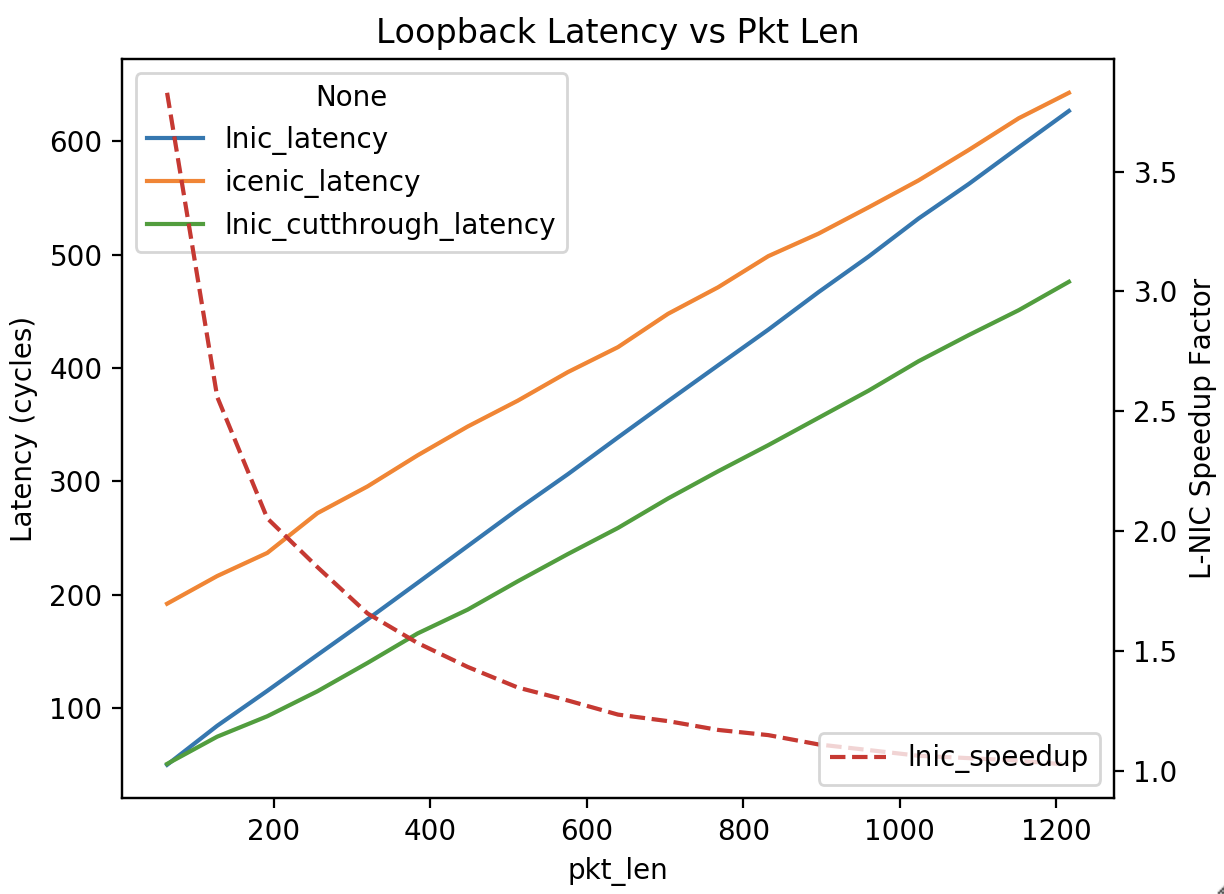
\includegraphics[width=\linewidth]{./figures/loopback-latency}
  \caption{NanoPU vs Traditional net-core-net loopback latency for various packet sizes.}
  \label{fig:loopback-latency}
\end{figure}

\paragraph{Basic NanoKernel Performance Analaysis.}
\begin{itemize}
    \item NanoKernel context switch latency
\end{itemize}

\subsection{Bare Metal Application Evaluations}
\begin{itemize}
    \item This section shows the reduction in average latency as a result of the hardware fast path to the core of the CPU.
    \item Streaming application (NFV style)
    \item Neural Network inference node
    \item Othello
    \item N-body simulation
\end{itemize}

\begin{figure}
  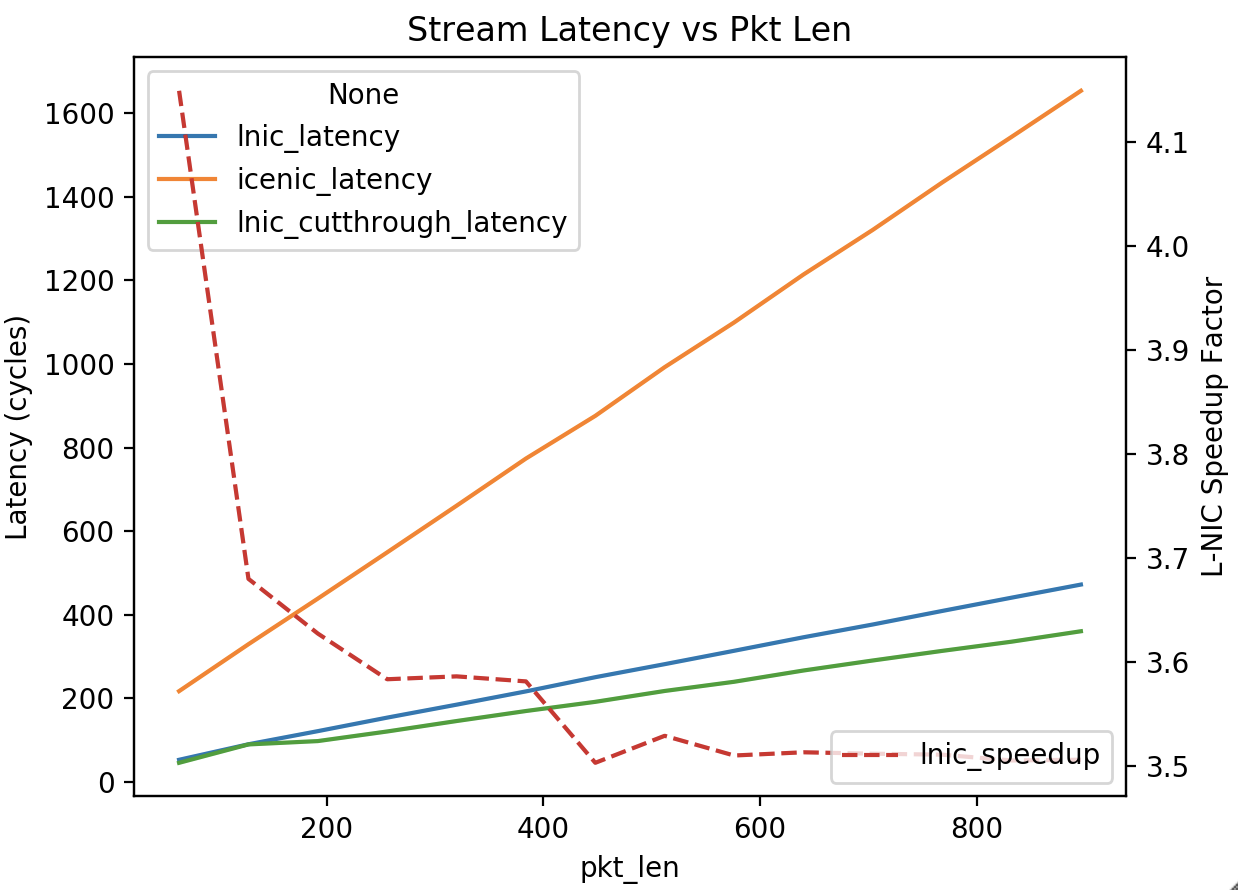
\includegraphics[width=\linewidth]{./figures/stream-latency}
  \caption{NanoPU vs Traditional NFV-style streaming application latency for various packet sizes.}
  \label{fig:stream_latency}
\end{figure}

\begin{figure}
  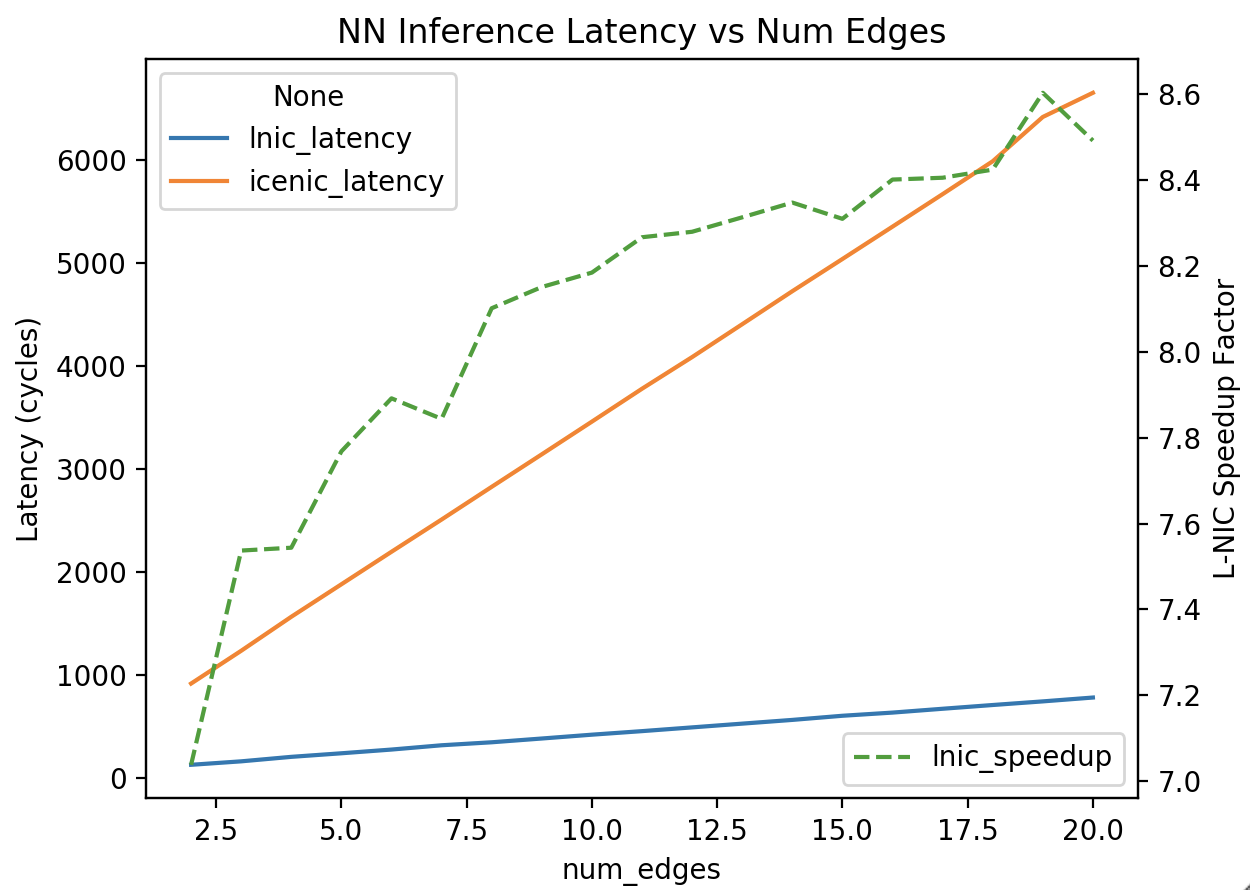
\includegraphics[width=\linewidth]{./figures/nn-inference-latency}
  \caption{NanoPU vs Traditional neural network node latency for various number of incoming edges.}
  \label{fig:nn_latency}
\end{figure}

\begin{figure}
  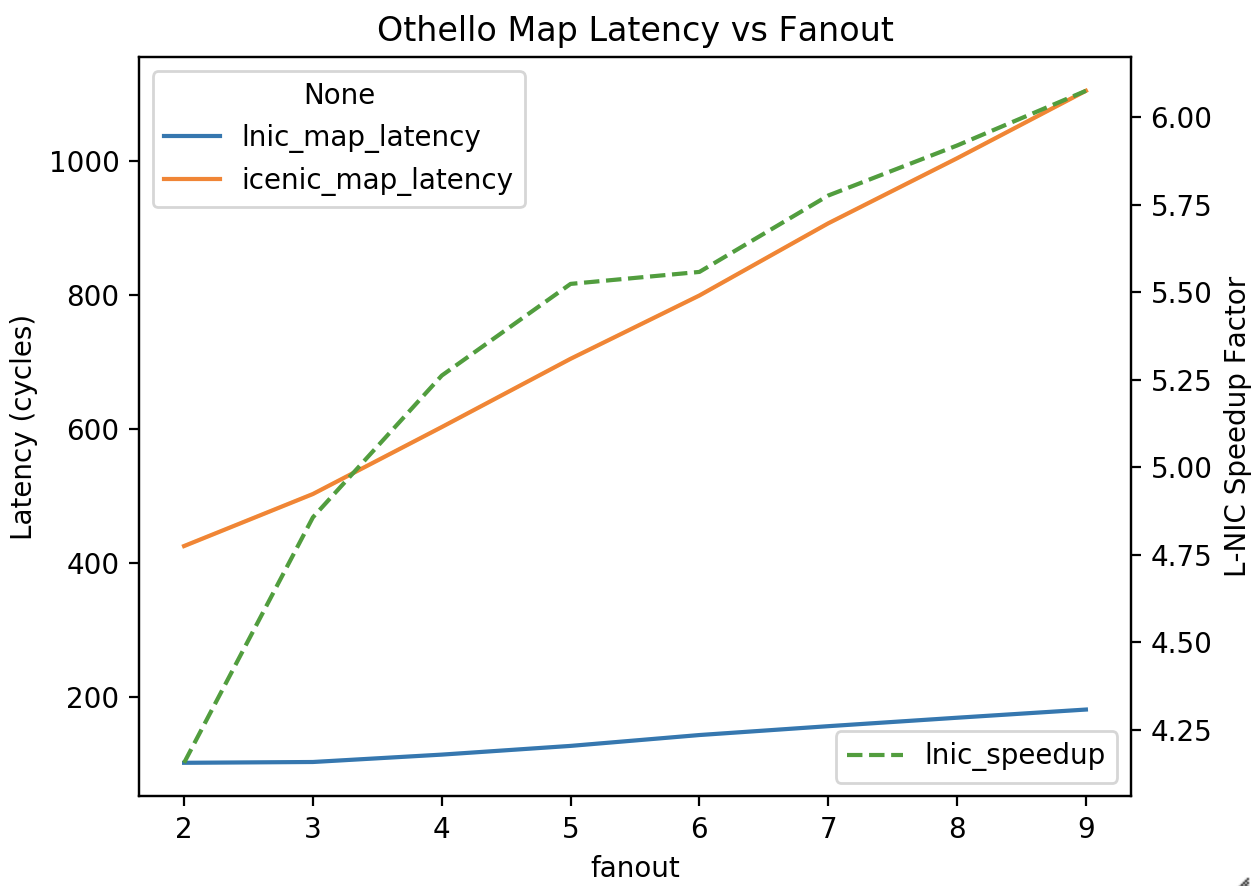
\includegraphics[width=\linewidth]{./figures/othello-map-latency}
  \caption{NanoPU vs Traditional Othello map latency for various degrees of fanout.}
  \label{fig:othello_map_latency}
\end{figure}

\begin{figure}
  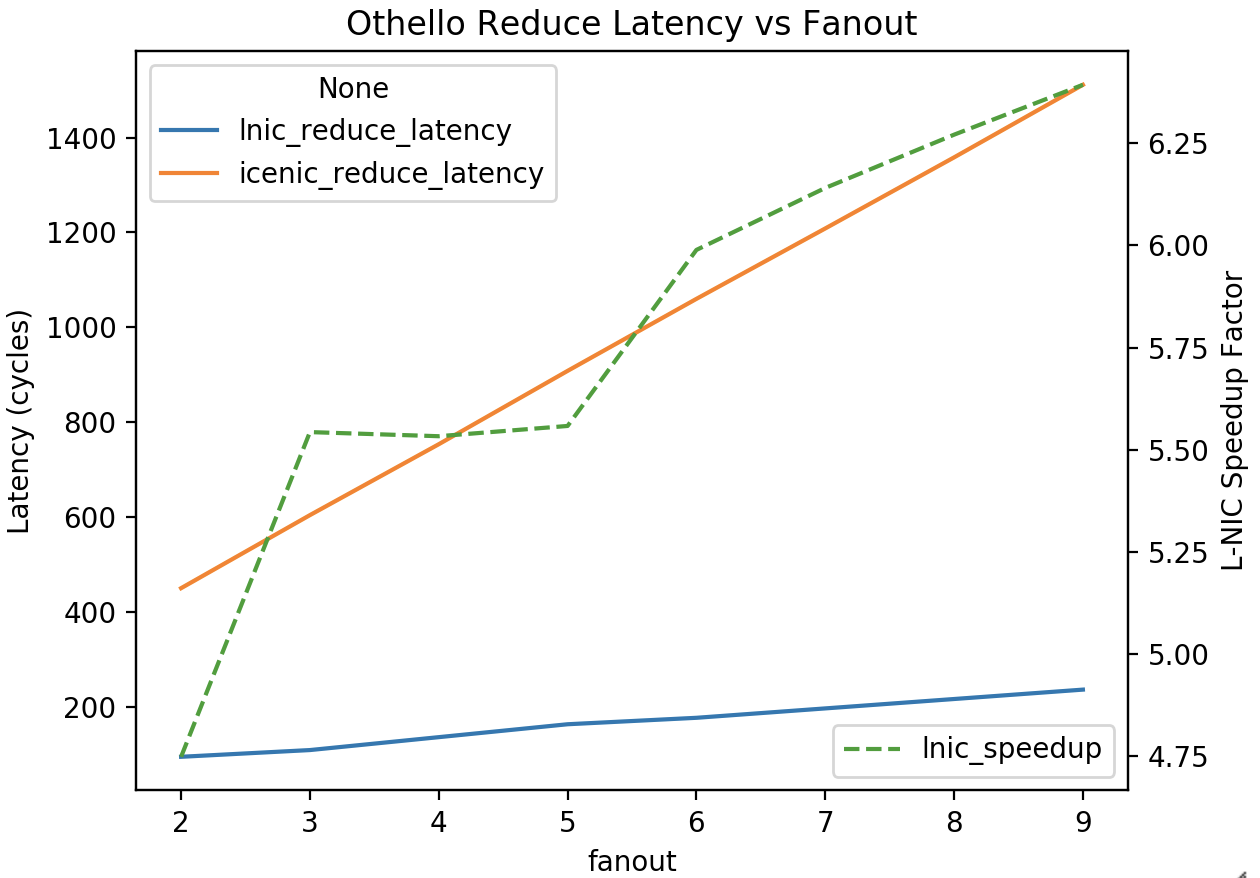
\includegraphics[width=\linewidth]{./figures/othello-reduce-latency}
  \caption{NanoPU vs Traditional Othello reduce latency for various degrees of fanout.}
  \label{fig:othello_reduce_latency}
\end{figure}

\subsection{Thread Scheduling Evaluations}
\begin{itemize}
    \item This section shows the reduction in tail latency as a result of NIC-driven thread scheduling for nanoservice applications.
    \item Compare Linux-style timer interrupt driven scheduling to NIC driven thread scheduling on the NanoPU.
    \item Explain the experiment set up.
    \item Show that NIC driven scheduling has much lower tail latency.
\end{itemize}

\subsection{Large Scale Nanoservice Evaluation}
\begin{itemize}
    \item Show evaluations of large scale (1000's of NanoPU cores) nanoservice deployment being used to implement an N-body simulation.
    \item Maybe compare to ChanGa.
    \item Show that the nanoservices implementation can perform the simulation much faster.
\end{itemize}
\section{Reproducibility}

Our \name{} prototype will be made publicly available along with all of our nanoservice application code and testing framework.
Additionally, we will make it very easy for anyone to reproduce all of our results by providing a virtual machine pre-installed with all the necessary dependencies, the prototype, and the tests.
\section{Discussion}
This section discusses a few additional details about the \name{}'s NIC-Core interface, as well as some thoughts regarding the \name{} as a domain specific processor and using it to run nanoservice applications.

\subsection{\name{} NIC-Core Interface Design Considerations}
As mentioned in \S\ref{sec:prototype}, the changes to the RISC-V Rocket core that were required to support our fast path to the register file were very minimal.
The most significant change resulted from the fact that reading the network RX queue in the CPU pipeline's decode stage causes a state change which must be undone when there is a pipeline flush resulting from a branch misprediction.
We handle this situation by simply modifying the RX queue to be able to effectively ``unread'' the last two words that were removed.

Our \name{} design reserves two general purpose registers for the head and tail of the network RX and TX queues respectively.
We also explored an alternative design where the head and tail registers are instead implemented using control status registers (CSRs).
This design decision of whether to use GPRs or CSRs has a number of trade offs.
Using GPRs often results in lower latency for applications because GPR values feed directly into the CPU's ALU and thus avoids the need to copy every word of every message from the CSR to a GPR before using the ALU.
However, if the number of GPRs is very limited, for example in a light weight embedded system, then sacrificing two GPRs may result in an excessive amount of register spill into memory, thus inflating latency.
Our experiments suggest that reducing the number of GPRs in the RISC-V Rocket core from 32 to 30, does not have a significant impact on the amount of register spill for our benchmark suite of nanoservice applications.

Our \name{} prototype is built on top of the RISC-V Rocket core, which is a simple 5-stage, in-order RISC processor.
While our prototype required very minor modifications to the CPU pipeline, the changes may need to be more invasive on an out-of-order RISC processor in order to ensure that words are read from the RX queue in the correct order.

Our \name{} design is optimized to minimize the latency from the network into the \emph{integer} register file.
Many scientific computing applications, such as the N-body simulation described in \S\ref{ssec:bare-metal-evals}, require use of messages with \emph{floating point} numbers.
Since the RISC-V ISA does not define instructions to directly copy bytes from an integer register to a floating point register without converting the number format, the number must first be stored into memory and then loaded into the floating point register file, resulting in additional latency.
We advocate for a minor change to the RISC-V ISA in order to support instructions that directly copy bytes between the integer and floating point register files.

\subsection{\name{} as a Domain Specific Processor}
We consider our \name{} prototype to be a first step towards building a domain specific processor for compute-intensive distributed applications.
In this paper, we focus on what we believe to be the most important components of the architecture: the network interface and thread scheduler.
That being said, we believe that future research on this topic should consider tailoring other aspects of the architecture including the memory hierarchy, on-chip network, CPU pipeline, and ISA for compute-intensive distributed applications.

Furthermore, it is not clear that writing C code is the best way to program the \name{}. Network applications written for the \name{} must process message data in FIFO order, have minimal memory requirements, and all communication is done via explicit message passing.
Perhaps there is a higher-level domain specific language that developers can use to facilitate writing stateful message processing applications. This could be an area of interesting research.

As a result of being a domain specific processor, there are classes of applications that we believe to be ill-suited for the \name{}, such as \emph{memory-intensive} distributed applications.
For example, a Key-Value store application~\cite{memcached} may or may not be well suited for the \name{}, depending on the scale and latency requirements.
If the size of the database is small enough to fit in the L1 caches of a reasonable amount of \name{} cores then it would likely be good fit and would provide substantially lower latency than a DRAM based Key-Value store.
However, if the size of the database is very large, then the \name{}'s fast path will probably not provide much benefit, although the \name{}'s NIC-driven scheduling policy may still be beneficial.

\subsection{Running Nanoservice Applications}
Rather than using a standard Linux distribution to test our scheduling policies we decided to use a minimal operating system of our own design - the nanoKernel.
Our main reason for doing this was to eliminate all of the general purpose logic in Linux in an effort to measure the minimum possible scheduling latency.
That being said, our current nanoKernel implementation is lacking a few Linux features that we believe would be beneficial for running nanoservice applications.
This includes features such as virtual memory and multiple privilege modes.
That is, all applications in the nanoKernel currently execute in the same address space and at the same privilege level.
We expect that this will change in future iterations of the nanoKernel.

In addition to the nanoKernel and hardware thread scheduler, we suspect that we may also need a runtime system that ensures the high utilization of \name{} cores and NICs.
This runtime system would be responsible for dispatching nanoservice apps to \name{} cores, monitoring the utilization of the cores and NICs, along with the status of contexts.
If some cores or NICs are over/under-utilized for a long period of time, it will need to rebalance the system.
If some contexts are starved for a long period of time, again it may need to address this.

% \begin{itemize}
%     \item The number of nanoservice apps running on any one core will likely be small in order to ensure that all the code and data resides in on-chip SRAM. Thus, we believe that it is feasible for the NIC to maintain per-context queues in hardware.
%     \item Mention that our prototype will be open sourced and all of our results will be made reproducible.
% \end{itemize}
\section{Related Work}
Smart NICs (i.e. NICs with CPUs on them) have become a popular trend recently~\cite{nitro, bluefield, pensando}.
They are hell bent on offloading processing logic in order to free up the host CPUs so that those cycles can be sold to paying customers.
Smart NICs are terrible for latency sensitive applications, in fact, they increase latency.
In order to make nanoservices practical, we believe that the NIC should be a domain specific architecture designed to minimize latency to the core, perform thread scheduling, and implement a transport protocol.
Throwing a CPU on a NIC is not what we would consider to be a domain specific architecture.

Microservices and serverless compute~\cite{aws-lambda, gcloud-functions, azure-functions} is another recent trend that enables developers to implement applications in a more fine grained manner than has every been feasible in the past.
Serverless compute infrastructure has been used to implement fine grained video encoding~\cite{ExCamera}, compilers~\cite{gg}, and scientific computing applications~\cite{PyWren}.
The nanoservices framework takes this approach to the absolute extreme and we believe that the nanoPU will help make this practical.

There are are number of recent works that attempt to minimize tail RPC completion time: Shinjuku~\cite{shinjuku}, Shenango~\cite{shenango}, RPCValet~\cite{rpcvalet}.
These works assume that incoming requests must be load balanced across cores.
We believe that this assumption will generally be false for the vast majority of nanoservice applications.
For the most part, nanoserver threads will need to directly send messages between one another.
That is, each message will indicate its destination thread ID and hence the core ID.
This is because in most cases, only one thread will have the state needed to processes a certain message.
That being said, there will be some nanoservice apps that will want to send messages which can be processed by any one of $N$ replicas.
In this situation, we believe that the load balancing decision should be made at the sending machine or within the network, not on machine(s) where the replicas reside.
One reason for this belief because the replicas many not even reside on the same machine, much less attached to the same NIC.
Another reason for this belief is that load balancing decisions made at the destination machine are already too late, especially with the massive degrees of incast that we expect nanoservices to exhibit.
Ideally, the nanoserver thread that is about to send the message will be aware of who is about to send a message to each replica so that it can make the most informed load balancing decision or perhaps decide to delay sending the message in the first place in order to avoid drops within the network or the destination NIC, wasting network bandwidth.
This would require an immense amount of coordination, which is perhaps achievable with tightly synchronized clocks across all machines.
This is our current area of active research.

We are not the first to propose an integrated network interface.
Scale-Out NUMA~\cite{scale-out-numa} integrates the network interface into the machine's local cache coherence hierarchy in order to accelerate RDMA style applications.
This approach is similar in spirit to the recent Compute Express Link (CXL)~\cite{cxl} standard, which is designed to maintain memory coherence between the CPU memory and the memory on PCIe attached devices.
Both of these approaches are sub-optimal for nanoservice applications, which require minimal latency between the network and the CPU pipeline, not memory.
Thus, the nanoPU integrates the network interface and the CPU pipeline.

The design of the nanoPU's network fast path into the CPU register file is inspired by the J-machine~\cite{jmachine} from 1989.
This machine proposed to communicate between processors on the same chip via the register file in order to minimize inter-processor communication latency.
The approach was eventually abandoned because it was believed to be challenging to maintain isolation between contexts running on the same core.
We believe that our proposal to use per-context queues in NIC hardware overcomes this challenge.


\section{Conclusion}
There are several conclusions to draw from this extreme approach to distributed computing. 
On one hand, the \name{} suggests a fairly simple, low-cost, non-invasive way to modify a CPU+NIC to accelerate distributed applications that can exploit very fine-grained nanotasks. 
We could expect dramatic speedups for this class of applications. 
On the other hand, one might dismiss nanoservices as too fine-grained for the remaining broad class of applications that require accesses to large pools of memory; these are unlikely to benefit from nanoservices because they cannot be cache resident. 

We envisage three deployment scenarios: First, racks of \name{}s in an otherwise unchanged datacenter, to which nanoservice jobs are directed. 
A single chip might contain over a thousand \name{} cores sharing over a hundred on-chip low-latency L-NIC interfaces. 
This would be a formidable platform for running nanoservice applications. 
Further, one can imagine extending stream processing and load-balancing into the NIC pipeline and network switches, offloading the CPU cores from processing tasks better suited to in-network computation. 
The second scenario is where an existing CPU has the \name{} features added to it, in addition to its normal cache, DRAM, DMA and PCIe hardware. 
In this case, the NIC would steer nanoservice RPC messages directly to the registers, while steering legacy network traffic via DMA into memory. 
A third scenario is for embedded applications, for example the CPUs on a modern smart NIC. 
These could be designed as a \name{} either to accelerate control of the smart NIC, or to host nanoservices to offload the end-host server. 
All three scenarios are technically possible. \chang{I'm not quite sure about this third use case. Isn't the s/w running in the control-plane of a smart NIC more memory bound? E.g., OVSDB. Hosting nanoservices to offload the host server sounds more compelling because, location wise, a smart NIC is just perfect.}

Our \name{} prototype design indicates that in all three scenarios, nanoservice applications would run several times faster, with more predictable completion times.
%\nick{check out this last paragraph. Not super happy with it; feel free to improve.}


\label{lastpage}

{\footnotesize 
\bibliographystyle{acm}
\bibliography{reference}
}

\label{totalpage}

\end{document}